\documentclass{wissdoc}

% Autor: Roland Bless 1996-2009, bless <at> kit.edu
% ----------------------------------------------------------------
% Diplomarbeit - Hauptdokument
% ----------------------------------------------------------------
%%
%% $Id: diplarb.tex 53 2009-12-10 12:23:37Z bless $
%%
% wissdoc Optionen: draft, relaxed, pdf --> siehe wissdoc.cls
% ------------------------------------------------------------------
% Weitere packages: (Dokumentation dazu durch "latex <package>.dtx")
\PassOptionsToPackage{hyphen}{url}
\usepackage{amssymb}
\usepackage{amsmath}
%\usepackage{bibgerm}
\usepackage[backend=bibtex,natbib=true]{biblatex}
\usepackage{booktabs}
\usepackage{boxhandler}
\usepackage{caption}
\usepackage{csquotes}
\usepackage{enumitem}
%\usepackage{fancybox} % für schattierte,ovale Boxen etc.
\usepackage{float}    %z.B. \floatstyle{ruled}\restylefloat{figure}
\usepackage[T1]{fontenc}
\usepackage{footnote}
\makesavenoteenv{table}
\makesavenoteenv{tabularx}
\usepackage{graphicx}
\usepackage[space]{grffile}
%\usepackage[plainpages=true]{hyperref}
%\usepackage{hyperref}
\usepackage{listings}
\usepackage{lscape}
\usepackage{multirow}
%\usepackage[numbers,sort&compress]{natbib}
\usepackage{newfloat,caption}
\usepackage{pdfpages}
\usepackage{pgfplotstable}
\usepackage{pgfplots}
\usepackage{rotating}
\usepackage{siunitx}
\usepackage{subcaption}
%\usepackage{subfig}
%\usepackage{subfigure}
%\usepackage{supertab} % mehrseitige Tabellen
%\usepackage[svnon,svnfoot]{svnver} % SVN Versionsinformation
\usepackage{tabularx}
\usepackage{tabu}
\usepackage{textcomp}
%\usepackage{tocbibind}
\usepackage{url}
%\usepackage{varioref}
%\usepackage{verbatim}
%\usepackage{xcolor}
%% ---------------- end of usepackages -------------

%\svnversion{$Id: diplarb.tex 53 2009-12-10 12:23:37Z bless $} % In case that you want to include version information in the footer
%\hyphenation{if...-then...}
%% Informationen für die PDF-Datei
\pgfplotsset{compat=newest}

\newsavebox{\Author}
\savebox{\Author}{Christian Navolskyi}

\newsavebox{\Title}
\savebox{\Title}{Benchmarking of Graph Databases - Suitability for the Industrial Environment}

\hypersetup{
%%% styling of link inside pdf
	colorlinks,
  citecolor=black,
  filecolor=black,
  linkcolor=black,
  urlcolor=black,
%%%
 pdfauthor={\usebox{\Author}},
 pdftitle={\usebox{\Title}}
 pdfsubject={Not set},
 pdfkeywords={Not set}
}
\DeclareFloatingEnvironment[fileext=frm,placement={!ht},name=Listing,within=section]{listing}

% Macros, nicht unbedingt notwendig
%%%%%%%%%%%%%%%%%%%%%%%%%%%%%%%%%%%%%%%%%%%%%%%%%%%%%%%%%%
% macros.tex -- einige mehr oder weniger nuetzliche Makros
% Autor: Roland Bless 1998
%%%%%%%%%%%%%%%%%%%%%%%%%%%%%%%%%%%%%%%%%%%%%%%%%%%%%%%%%%
% $Id: macros.tex 33 2007-01-23 09:00:59Z bless $
%%%%%%%%%%%%%%%%%%%%%%%%%%%%%%%%%%%%%%%%%%%%%%%%%%%%%%%%%%


%%%%%%%%%%%%%%%%%%%%%%%
% Kommentare 
%%%%%%%%%%%%%%%%%%%%%%%
\ifnotdraftelse{
\newcommand{\Kommentar}[1]{}
}{\newcommand{\Kommentar}[1]{{\em #1}}}
% Alles innerhalb von \Hide{} oder \ignore{} 
% wird von LaTeX komplett ignoriert (wie ein Kommentar)
\newcommand{\Hide}[1]{}
\let\ignore\Hide

%%%%%%%%%%%%%%%%%%%%%%%%%
% Leere Seite ohne Seitennummer, wird aber gezaehlt
%%%%%%%%%%%%%%%%%%%%%%%%%

\newcommand{\leereseite}{% Leerseite ohne Seitennummer, nächste Seite rechts (wenn 2-seitig)
 \clearpage{\pagestyle{empty}\cleardoublepage}
}
%%%%%%%%%%%%%%%%%%%%%%%%%%
% Flattersatz rechts und Silbentrennung, Leerraum nach rechts maximal 1cm
%%%%%%%%%%%%%%%%%%%%%%%%%%
\makeatletter
\newcommand{\myraggedright}{%
 \let\\\@centercr\@rightskip 0pt plus 1cm
 \rightskip\@rightskip
  \leftskip\z@skip
  \parindent\z@
  \spaceskip=.3333em
  \xspaceskip=.5em}
\makeatother

\makeatletter
\newcommand{\mynewline}{%
 \@centercr\@rightskip 0pt plus 1cm
}
\makeatother


%%%%%%%%%%%%%%%%%%%%%%%%%%
% Für Index
%%%%%%%%%%%%%%%%%%%%%%%%%%
\makeatletter
\def\mydotfill{\leavevmode\xleaders\hb@xt@ .44em{\hss.\hss}\hfill\kern\z@}
\makeatother
\def\bold#1{{\bfseries #1}}
\newbox\dbox \setbox\dbox=\hbox to .4em{\hss.\hss} % dot box for leaders
\newskip\rrskipb \rrskipb=.5em plus3em % ragged right space before break
\newskip\rrskipa \rrskipa=-.17em plus -3em minus.11em % ditto, after
\newskip\rlskipa \rlskipa=0pt plus3em % ragged left space after break
\newskip\rlskipb \rlskipb=.33em plus-3em minus.11em % ragged left before break
\newskip\lskip \lskip=3.3\wd\dbox plus1fil minus.3\wd\dbox % for leaders
\newskip \lskipa \lskipa=-2.67em plus -3em minus.11em %after leaders
\mathchardef\rlpen=1000 \mathchardef\leadpen=600
\def\rrspace{\nobreak\hskip\rrskipb\penalty0\hskip\rrskipa}
\def\rlspace{\penalty\rlpen\hskip\rlskipb\vadjust{}\nobreak\hskip\rlskipa}
\let\indexbreak\rlspace
\def\raggedurl{\penalty10000 \hskip.5em plus15em \penalty0 \hskip-.17em plus-15em minus.11em}
\def\raggeditems{\nobreak\hskip\rrskipb \penalty\leadpen \hskip\rrskipa %
\vadjust{}\nobreak\leaders\copy\dbox\hskip\lskip %
\kern3em \penalty\leadpen \hskip\lskipa %
\vadjust{}\nobreak\hskip\rlskipa}
\renewcommand*\see[2]{\rlspace\emph{\seename}~#1} % from makeidx.sty

%%%%%%%%%%%%%%%%%%%%%%%%%%
% Neue Seite rechts, leere linke Seite ohne Headings
%%%%%%%%%%%%%%%%%%%%%%%%%%
\newcommand{\xcleardoublepage}
{{\pagestyle{empty}\cleardoublepage}}

%%%%%%%%%%%%%%%%%%%%%%%%%%
% Tabellenspaltentypen (benoetigt colortbl)
%%%%%%%%%%%%%%%%%%%%%%%%%%
\newcommand{\PBS}[1]{\let\temp=\\#1\let\\=\temp}
\newcolumntype{y}{>{\PBS{\raggedright\hspace{0pt}}}p{1.35cm}}
\newcolumntype{z}{>{\PBS{\raggedright\hspace{0pt}}}p{2.5cm}}
\newcolumntype{q}{>{\PBS{\raggedright\hspace{0pt}}}p{6.5cm}}
\newcolumntype{g}{>{\columncolor[gray]{0.8}}c} % Grau
\newcolumntype{G}{>{\columncolor[gray]{0.9}}c} % helleres Grau

%%%%%%%%%%%%%%%%%%%%%%%%%%
% Anführungszeichen oben und unten
%%%%%%%%%%%%%%%%%%%%%%%%%%
\newcommand{\anf}[1]{"`{#1}"'}

%%%%%%%%%%%%%%%%%%%%%%%%%%
% Tiefstellen von Text
%%%%%%%%%%%%%%%%%%%%%%%%%%
% S\tl{0} setzt die 0 unter das S (ohne Mathemodus!)
% zum Hochstellen gibt es uebrigens \textsuperscript
\makeatletter
\DeclareRobustCommand*\textlowerscript[1]{%
  \@textlowerscript{\selectfont#1}}
\def\@textlowerscript#1{%
  {\m@th\ensuremath{_{\mbox{\fontsize\sf@size\z@#1}}}}}
\let\tl\textlowerscript
\let\ts\textsuperscript
\makeatother

%%%%%%%%%%%%%%%%%%%%%%%%%%
% Gauß-Klammern
%%%%%%%%%%%%%%%%%%%%%%%%%%
\newcommand{\ceil}[1]{\lceil{#1}\rceil}
\newcommand{\floor}[1]{\lfloor{#1}\rfloor}

%%%%%%%%%%%%%%%%%%%%%%%%%%
% Average Operator (analog zu min, max)
%%%%%%%%%%%%%%%%%%%%%%%%%%
\def\avg{\mathop{\mathgroup\symoperators avg}}

%%%%%%%%%%%%%%%%%%%%%%%%%%
% Wortabkürzungen
%%%%%%%%%%%%%%%%%%%%%%%%%%
\def\zB{z.\,B.\ }
\def\dh{d.\,h.\ }
\def\ua{u.\,a.\ }
\def\su{s.\,u.\ }
\newcommand{\bzw}{bzw.\ }

%%%%%%%%%%%%%%%%%%%%%%%%%%%%%%%%%%%
% Einbinden von Graphiken
%%%%%%%%%%%%%%%%%%%%%%%%%%%%%%%%%%%
% global scaling factor
\def\gsf{0.9}
%% Graphik, 
%% 3 Argumente: Datei, Label, Unterschrift
\newcommand{\Abbildung}[3]{%
\begin{figure}[tbh] %
\centerline{\scalebox{\gsf}{\includegraphics*{#1}}} %
\caption{#3} %
\label{#2} %
\end{figure} %
}
\let\Abb\Abbildung
%% Abbps
%% Graphik, skaliert, Angabe der Position
%% 5 Argumente: Position, Breite (0 bis 1.0), Datei, Label, Unterschrift
\newcommand{\Abbildungps}[5]{%
\begin{figure}[#1]%
\begin{center}
\scalebox{\gsf}{\includegraphics*[width=#2\textwidth]{#3}}%
\caption{#5}%
\label{#4}%
\end{center}
\end{figure}%
}
\let\Abbps\Abbildungps
%% Graphik, Angabe der Position, frei wählbares Argument für includegraphics
%% 5 Argumente: Position, Optionen, Datei, Label, Unterschrift
\newcommand{\Abbildungpf}[5]{%
\begin{figure}[#1]%
\begin{center}
\scalebox{\gsf}{\includegraphics*[#2]{#3}}%
\caption{#5}%
\label{#4}%
\end{center}
\end{figure}%
}
\let\Abbpf\Abbildungpf

%%
% Anmerkung: \resizebox{x}{y}{box} skaliert die box auf Breite x und Höhe y,
%            ist x oder y ein !, dann wird das usprüngliche 
%            Seitenverhältnis beibehalten.
%            \rescalebox funktioniert ähnlich, nur das dort ein Faktor
%            statt einer Dimension angegeben wird.
%%
% \Abbps{Position}{Breite in Bruchteilen der Textbreite}{Dateiname}{Label}{Bildunterschrift}
%

\newcommand{\refAbb}[1]{%
s.~Abbildung \ref{#1}}

%%%%%%%%%%%%%%%%%%%%
%% end of macros.tex
%%%%%%%%%%%%%%%%%%%%

% Print URLs not in Typewriter Font
\def\UrlFont{\rm}

\newcommand{\specialcell}[2][c]{%
  \begin{tabular}[#1]{@{}c@{}}#2\end{tabular}}

%\newcommand\todo[1]{\textcolor{red}{}}
\newcommand\todo[1]{\textcolor{red}{TODO: #1}}

%\newcommand\note[1]{\textcolor{blue}{}}
\newcommand\note[1]{\textcolor{blue}{NOTE: #1}}

\newcommand\hlcode[1]{\textcolor{red}{#1}}

\newcommand\citeable[1]{\textcolor{green}{\hl{citeable: #1}}}

\newcolumntype{$}{>{\global\let\currentrowstyle\relax}}
\newcolumntype{^}{>{\currentrowstyle}}
\newcommand{\rowstyle}[1]{\gdef\currentrowstyle{#1}%
  #1\ignorespaces
}

\newif\ifcomment
%\commenttrue %# Show comments


\newcommand{\blankpage}{% Leerseite ohne Seitennummer, nächste Seite rechts
 \clearpage{\pagestyle{empty}\cleardoublepage}
}

%% Einstellungen für das gesamte Dokument

% Trennhilfen
% Wichtig!
% Im german-paket sind zusätzlich folgende Trennhinweise enthalten:
% "- = zusätzliche Trennstelle
% "| = Vermeidung von Ligaturen und mögliche Trennung (bsp: Schaf"|fell)
% "~ = Bindestrich an dem keine Trennung erlaubt ist (bsp: bergauf und "~ab)
% "= = Bindestrich bei dem Worte vor und dahinter getrennt werden dürfen
% "" = Trennstelle ohne Erzeugung eines Trennstrichs (bsp: und/""oder)

% Trennhinweise fuer Woerter hier beschreiben
\hyphenation{
% Pro-to-koll-in-stan-zen
% Ma-na-ge-ment  Netz-werk-ele-men-ten
% Netz-werk Netz-werk-re-ser-vie-rung
% Netz-werk-adap-ter Fein-ju-stier-ung
% Da-ten-strom-spe-zi-fi-ka-tion Pa-ket-rumpf
% Kon-troll-in-stanz
}
\lstset{
    frame=single,
    breaklines=true,
		basicstyle=\scriptsize,
    %postbreak=\raisebox{0ex}[0ex][0ex]{\ensuremath{\color{red}\hookrightarrow\space}}
}

% Index-Datei öffnen
\ifnotdraft{\makeindex}
%%%%%%%%%%%%%% includeonly %%%%%%%%%%%%%%%%%%%
% Es werden nur die Teile eingebunden, die hier
% aufgefuehrt sind!
%\includeonly{%
%titlepage,%
%statement,% Ist in KA Pflicht für Diplomarbeiten
%introduction,% Motivation, Zielsetzung, Gliederung
%background,% Grundlagen
%analysis,   % Problembeschreibung (Detail) und Related Work
%design,   % Beschreibung der Problemlösung (Konzepte, allg. Architektur, ...)
%implementation,  % Beschreibung der Umsetzung/Implementierung
%evaluation,      % Nachweis und Auswertung
%futurework,% Future Work
%summary  % Zusammenfassung der Ergebnisse
%}
\bibliography{library,Websites}
\usepgfplotslibrary{groupplots}
\usetikzlibrary{pgfplots.groupplots}
%\addbibresource{diplarb.bib}

%%%%%%%%%%%%%%%%%%%%%%%%%%%%%%%%%%%%%%%%%%%%%%
\begin{document}

\frontmatter
\pagenumbering{roman}

\ifnotdraft{
%	\begin{titlepage}
%		
\includepdf[pages=1]{Deckblatt_Navolskyi}
%		\blankpage
%		
\includepdf[pages=2]{Deckblatt_Navolskyi}
%	\end{titlepage}
 %% Titelseite
%% Vorlage $Id: titelseite.tex 54 2009-12-10 12:23:58Z bless $

\def\usesf{}
\let\usesf\sffamily % diese Zeile auskommentieren für normalen TeX Font

\newsavebox{\Erstgutachter}
\savebox{\Erstgutachter}{\usesf Prof.~Dr.~Michael Beigl}
\newsavebox{\Zweitgutachter}
\savebox{\Zweitgutachter}{\usesf \todo{Eintragen}}

\begin{titlepage}
\setlength{\unitlength}{1pt}

\begin{picture}(0,0)(85,770)

\includegraphics[width=\paperwidth]{logos/KIT_Deckblatt}
\end{picture}

\vspace*{-39pt}\hspace*{300pt}
\includegraphics[width=.27\paperwidth]{logos/TECO_KIT}

\thispagestyle{empty}

%\begin{titlepage}
%%\let\footnotesize\small \let\footnoterule\relax
\begin{center}
\hbox{}
\vfill
{\usesf
{\huge\bfseries Totally Awesome Title of the Thesis
 \par}
\vskip 1.8cm
Master's Thesis\\
by\\[2mm]
\vskip 1cm

{\large\bfseries FirstName LastName\\}
\vskip 1.2cm
Chair of Pervasive Computing Systems/TECO\\
Institute of Telematics\\
Department of Informatics\\
%Universität Karlsruhe (TH)\\[2ex]
\vskip 3cm
\begin{tabular}{p{5.5cm}l}
First Reviewer: & \usebox{\Erstgutachter} \\
Second Reviewer: & \usebox{\Zweitgutachter} \\
Supervisor: & Name of Supervisor \\
\end{tabular}
\vskip 3cm
Project Period:\qquad 01/01/1970 -- XX/XX/20XX
}
\end{center}
\vfill
\end{titlepage}
%% Titelseite Ende


%%% Local Variables: 
%%% mode: latex
%%% TeX-master: "diplarb"
%%% End: 

	\blankpage % Leerseite auf Titelrückseite
	%
	% Die folgende Erklärung ist für Diplomarbeiten Pflicht
	% (siehe Prüfungsordnung), für Studienarbeiten nicht notwendig
	\thispagestyle{empty}
\vspace*{37\baselineskip}
\hbox to \textwidth{\hrulefill}
\par
\textbf{Erklärung}

Hiermit erkl\"are ich,
dass ich die vorliegende Bachelorarbeit selbstst\"andig verfasst und keine anderen als die angegebenen Hilfsmittel und Quellen benutzt habe,
die w\"ortlich oder inhaltlich \"ubernommenen Stellen als solche kenntlich gemacht und weiterhin die Richtlinien des KIT zur Sicherung guter wissenschaftlicher Praxis beachtet habe.

Karlsruhe, den 14.05.2018

\cleardoublepage


\chapter*{Zusammenfassung}

In dem derzeitigen Wandel der Industrie in Richtung Industrie 4.0 kommt es auch dazu,
dass viele Daten produziert werden,
welche wertvoll sind,
da sie für Verbesserungen in der Produktion verwendet werden können.
Die anfallenden Daten können als Graph repräsentiert werden,
deswegen macht es Sinn Graph-Datenbanken zu untersuchen.\\
In dieser Arbeit werden wir die Performanz von Graph-Datenbanken in einem industriellen Umfeld untersuchen.
Unser Ziel ist es,
herauszufinden ob die Resultate aus bestehender Forschung in diesem Gebiet herangezogen werden können um die Tauglichkeit der Graph-Datenbanken in der Industrie zu prüfen.
Anstatt Graphen ähnlich zu denen in sozialen Netzen für die Untersuchungen zu nutzen,
wie es die meisten Studien in diesem Gebiet tun,
werden wir eine Daten-Struktur entwerfen die den industriellen Datenraum repräsentiert und schauen uns ebenso die Besonderheiten eines industriellen Einsatzes einer Graph-Datenbank an,
um unsere Arbeits\-lasten entsprechend zu entwerfen.

Der Yahoo! Cloud Service Benchmark (YCSB) wird erweitert um Datensätze mit der von uns entworfenen Datenstruktur zu generieren.
Für die Auswertung haben wir folgende vier allgemein bekannte Graph-Datenbanken ausgewählt,
Apache Jena, Neo4j, OrientDB und Sparksee (früher bekannt unter dem Namen DEX).
Deren Java APIs wurden genutzt um sie in YCSB einzubinden.

Wir haben die Datenbanken mit unserer Datenstruktur auf einem einzelnen Rechner mit einem i7-3770K Prozessor und 16GB RAM ausgeführt und kamen zu dem Fazit,
dass aktuelle Graph-Datenbanken nicht für den industriellen Einsatz geeignet sind.\\
Sparksee konnte nicht mit dem Datensatz in voller Größe getestet werden,
da die kostenlose Lizenz diese Datenmenge nicht unterstützt.
Wenn es den erreichten Durchsatz halten könnte,
würde es auch mit dem Datenaufkommen aus der Industrie zurechtkommen.
Da wir das nicht direkt testen konnten,
können wir keine fundierte Entscheidung diesbezüglich treffen.
OrientDB verfehlte unser gesetztes Ziel für den Durchsatz nur knapp,
wohingegen Jena und Neo4j weit davon entfernt waren.\\
Nachdem wir die Generalisierbarkeit von Resultaten aus Graph-Datenbank Benchmarks ausgewertet haben,
können wir auch hier keine eindeutige Entscheidung treffen,
da Vergleiche mit unterschiedlichen Studien zu verschiedenen Schlussfolgerungen führen.
Wir konnten allerdings feststellen,
dass die Performanz beim hinzufügen von Knoten und Kanten unter anderem auch vom Lese-Durchsatz abhängt,
da diese Operation gebraucht wird,
um Kanten zum Graphen hinzuzufügen.
Schließlich scheinen jedoch mehr Argumente dafür zu sprechen,
dass Graph-Datenbanken schlechter im industriellen Einsatz abschneiden.
Das führt dazu,
dass die Resultate aus anderen Studien nicht direkt übernommen werden können.

\cleardoublepage

\chapter*{Abstract}

In the current transition happening in the industry towards Industry 4.0,
a lot of data is produced.
This data is valuable as it can be used for all kinds of improvements in the production process.
The accumulating data can be represented in a graph and therefore it is worth examining graph databases.\\
In this thesis,
we will investigate the performance of graph databases in an industrial environment.
Our goal is to examine whether the results of other research in the field of graph databases can be used to determine the performance of a graph database in the industrial internet of things.
Instead of using social network graphs as other research in this field does,
we will design a data structure that represents the industrial data space and also look at the peculiarities of an industrial use to design our workloads accordingly.

The YCSB benchmark will be extended to create datasets with our desired data structure.
For the benchmark,
we chose the following four commonly known graph databases, Apache Jena, Neo4j, OrientDB and Sparksee (also known as former DEX).
Their Java APIs were used to integrate them into YCSB.

We evaluated the databases with our data structure on a single machine with an i7-3770K processor and 16GB of RAM and came to the conclusion,
that graph databases aren't suitable for an industrial application.
Sparksee couldn't be tested with the large dataset,
due to a missing license.
If it could hold its throughput it would be suitable,
since we couldn't investigate that,
no solid conclusion can be drawn.
OrientDB missed the target throughput slightly,
whereas Jena and Neo4j were far away from the target throughput.\\
After evaluating the generalisability of graph database benchmark results we came to no clear conclusion,
as the comparison with other research points into two different directions.
However,
we can say that the insert throughput also depends on the read performance of the database as inserting edges requires read operations.
Besides that,
there were more arguments indicating that graph databases perform worse in an industrial environment.
This leads to the conclusion,
that the results of other studies cannot directly be used to determine the performance in an industrial use case.

\cleardoublepage

\blankpage % Leerseite auf Erklärungsrückseite
}
%
%% *************** Hier geht's ab ****************
%% ++++++++++++++++++++++++++++++++++++++++++
%% Verzeichnisse
%% ++++++++++++++++++++++++++++++++++++++++++
\ifnotdraft{
{\parskip 0pt\tableofcontents} % toc bitte einzeilig
%\pagenumbering{roman}
%\cleardoublepage
%\addcontentsline{toc}{chapter}{\listfigurename}
%\listoffigures
%
%\cleardoublepage
%\addcontentsline{toc}{chapter}{\listtablename}
%\listoftables
%\addcontensline{toc}{section}{List of Tables}
%\pagenumbering{roman}
%\listoffigures
%\addcontensline{toc}{section}{List of Figures}
%\blankpage
%\listoffigures
%\blankpage
%\listoftables
%\blankpage
}
\cleardoublepage
\blankpage

%% ++++++++++++++++++++++++++++++++++++++++++
%% Hauptteil
%% ++++++++++++++++++++++++++++++++++++++++++
\graphicspath{{images/}}

\mainmatter
\null
\newpage
\pagenumbering{arabic}
\chapter{Introduction}
\label{ch:introduction}
%% ==============================
% CLEARLY SHOW CONTRIBUTIONS AND LINK THEM TO SECTIONS

\todo{Fix url in bibliography}

\section{Problem Statement}
With the growing digitalisation of the industry,
more data is available and can be used to improve production processes.
The amount of data created depends on the individual use case but still,
it needs to be stored to be useful.
Since there are multiple databases available it can be difficult to choose the right one for an individual scenario.

Current graph database benchmark only cover social network graphs,
which differ from the data structure present in the industry in their edge to node ration as well as their cluster coefficient.

\subsection{Use Case - Industry 4.0}
There are multiple analytic algorithms to run on data to extract certain features.
In the industry,
those algorithms play an important role too but in this thesis we are looking at different aspects of the industrial use case,
mainly inserting data and reading data.
As far as we know an industrial data structure was not used to examine the performance of graph databases.

In section~\ref{ch:background:se:industrialData} we will show an example given by the industry.
There is no industrial data available publicly so we have to base our design on that given example which is visualised in figure~\ref{fig:exampleData}.

\subsubsection{Inserting Data}
To digitalise the production processes the data produced by every machine in the production line should be stored for future analysis.
And to store that data it needs to be written into a database.
Since most factories running 24 hours a day,
the machines are producing a lot of data during the day.
That will be the base load for the underlying database, to store all that data from the production machines.

\subsubsection{Reading Data}
Besides using the stored data for analysis algorithms,
simply reading data from the database is another common use case.
An example would be to get the time at which a specific product was processed by a specific machine to check if all parameters were set correctly.

\section{Question}
The question of our research is,
how well current graph databases are capable of handling the amount of data created in an industrial environment.
Furthermore we will look at how the structure effects performance to conclude if other research investigating the performance of graph databases can be used to determine the performance these databases would have in an industrial environment.

\section{Methodology}
We will chose the databases to use for our testing from other studies covering benchmarking graph databases to be able to compare the results and look to similarities in behaviour.
To evaluate different databases we first will look up existing benchmarks and choose the best fitting one for our research.
In the benchmarking program we need to look at the creation of data and how it can be stored and retrieved.
The same exact dataset should be used for all databases equally to eliminate the variation that comes with generating data during each benchmark run.
Workloads will be designed to investigate the performance of graph databases with industrial data and the production environment will be simulated.
With the databases and benchmark set up we will run the workloads and evaluate the results to conclude if current database are suitable for the industrial internet of things.

\section{Goal of this Thesis}
With this thesis we want to examine whether and if so,
how well graph databases are able to stand the load of an production line.
Because every manufacturer is different and we cannot cover all scenarios we try to cover the most important parameters
so that the suitability for the individual case can be estimated.
Besides this specific investigation we will try to conclude if the results of research performed on graph databases with social network graphs can be applied to the industrial use case.

\section{Structure}
In chapter~\ref{ch:background} we are motivating graph and the use of graph databases.
The different kinds of graph databases are explained and an example database which we are testing is mentioned and shortly described.
Also in this chapter we are comparing the different available benchmarking programs and their features and take a look at research done by others in the field of graph database benchmarking.

In chapter~\ref{ch:analysis} the industrial data is modelled and its structure is analysed as well as a reasonable amount of data is determined.
Then we are figuring out how a workload could look like in an industrial environment.
At last we further analyse out chosen benchmarking program and give an overview of its procedure.

Chapter~\ref{ch:design} is focused on the design of the different extensions for the benchmark and also the concrete data structure.
For the extension we cover the design of the specific workloads,
the design of classes to create and recreate the dataset,
the graph workload class managing the graph databases and the graph data and finally the database bindings which are responsible for connecting the database to the benchmarking program.

In chapter~\ref{ch:implementation} the implementation of the single components is described.
First we cover the graph data generator which includes the class for creating the graph data as well as the class for recreating it from files.
Next the bindings are implemented and their individual adaptions to the benchmark are highlighted.
And lastly we explain the graph workload class which is the mediator between the created graph data and the database bindings.

Chapter~\ref{ch:evaluation} focuses on running the benchmark and evaluating the results.
First, we define our objective during evaluation.
Then the configuration of our system is stated, as well as the hardware as the software side.
Next the procedure of running the benchmarks sequentially is explained following be the different aspects we are testing.
These are grouped into "throughput" in section~\ref{ch:evaluation:se:throughput}, "production simulation" in section~\ref{ch:evaluation:se:productionSimulation} and "retrieving under load" in section~\ref{ch:evaluation:se:retrievingUnderLoad}.
Each group includes multiple benchmarks in which we changed on variable at a time.
The results are presented directly after each benchmark followed by a discussion to interpret the results.

In chapter~\ref{ch:futureWork} we draw a conclusion over out work and give the answer to our question from above.
Also ideas for future research and development in this field are presented.
Finally a summary is given in the end of this chapter.
  % Einleitung
%% grundlagen.tex
%% $Id: grundlagen.tex 28 2007-01-18 16:31:32Z bless $
%%

\chapter{Background \& Related Work}
\label{ch:Background}

\section{Industrial Data}

\section{Graph Databases}

\section{Graph Database Benchmarks}

\section{Related Work}
  % Grundlagen
\chapter{Analysis}
\label{ch:analysis}
In this chapter we will analyse the data that could occur in an industrial use case,
including its structure and amount.
Further we will examine possible workloads for our graph databases in section~\ref{ch:analysis:se:workloads}.

At the end of this chapter in section~\ref{ch:analysis:se:benchmark} we will choose one benchmark for our research.

\section{Data}
\label{ch:analysis:se:data}
As described in section~\ref{ch:background:se:industrialData} we have to work with the data coming from production machines.
Figure~\ref{fig:exampleData} shows how that data could look like.

Additionally,
our partners at SICK AG~\cite{SICK} gave us the following key data of a product example.

\begin{itemize}
  \item A component carrier is produced every three minutes.
  \item A component carrier has up to 64 circuit boards.
  \item A circuit board has up to 128 components.
  \item A component is tested for up to 128 test features.
\end{itemize}

With this information we will calculate the amount of data in subsection~\ref{ch:analysis:se:dataAmount}

\subsection{Data Structure}
Looking at the graph in figure~\ref{fig:exampleData} and the example given by SICK we can see that the data looks much like a tree with some cross edges.
A root node at the top and multiple children connected to it with multiple children each.
The given excerpt from figure~\ref{fig:exampleData} shows a part of a testing procedure for a board with components.
Three properties of each component were observed.

We keep this structure in mind for our design in section~\ref{ch:design:se:dataStructure},
where we will compose the data structure for our implementation and evaluation.

\subsection{Data Amount}
\label{ch:analysis:se:dataAmount}
To evaluate the amount of data created during production we need to know how much is produced per time unit.
With the parameters mentioned in~\ref{ch:analysis:se:data} we can calculate the maximum number of data points produced every three minutes.

\begin{equation}
  \label{eq:dataAmount}
  \begin{aligned}
    n_{nodes} &= n_{componentCarrier} \\
    &\quad + n_{componentCarrier} \times n_{circuitBoard} \\
    &\quad + n_{componentCarrier} \times n_{circuitBoard} \times n_{component} \\
    &\quad + n_{componentCarrier} \times n_{circuitBoard} \times n_{component} \times n_{test} \\
    \iff &= 1 + 1 \times 64 + 1 \times 64 \times 128 + 1 \times 64 \times 128 \times 128 \\
    \iff &= 1 \times (1 + 64 + 64 \times 128 + 64 \times 128 \times 128) \\
    \iff &= 1 + 64 + 64 \times 128 + 64 \times 128 \times 128 \\
    \iff &= 1 + 64 \times (1 + 128 + 128 \times 128) \\
    \iff &= 1 + 64 \times (1 + 128 \times (1 + 128)) \\
    \iff &= 1 + 64 \times (1 + 128 \times 129) \\
    \iff &= 1 + 64 \times 16513 \\
    \iff &= 1056833
  \end{aligned}
\end{equation}

To calculate the target throughput the databases have to archive,
we need to know how many edges are between the different nodes.
Therefore,
we need a finished data structure.
In the next chapter in section~\ref{ch:design:se:suitability} we will calculate the target throughput in $ \frac{inserts}{s} $ for the workload design.

We can extract the size of each data point from our given example.
Each measurement is only two to three characters long,
however the other values range from $ 1 $ to around $ 75 $ characters.
The size for our workload should therefore be in that range.

\section{Workloads}
\label{ch:analysis:se:workloads}
Workloads should represent the mix of operations executed on a database.
There are two main uses for a database in an industrial environment,
the first one is described in section~\ref{ch:analysis:se:insertingData}.
Another one is presented in section~\ref{ch:analysis:se:retrievingData}.
The given examples are based on what we think would represent the industrial use of databases.

In section~\ref{ch:design:se:workloads} we will specify the workloads for our evaluation,
the following subsections should only motivate the specific use cases.

\subsection{Inserting Data into the Database}
\label{ch:analysis:se:insertingData}
It isn't rare that production runs 24h a day,
therefore data is produced all around the clock.
Because of that the ability to store data quickly is a decisive point in choosing a database.
As the machines operate,
data is continuously written to the database.

\subsection{Retrieving Data from the Database}
\label{ch:analysis:se:retrievingData}
Besides the previous mentioned continuous writing of data into the database,
retrieving data from the database would be the next common use for it.
That could be in the form of looking up a certain product produced in the past,
to retrieve its test parameter values or to get all products made by a specific machine to check if some are faulty.

\section{Benchmark Comparison}
\label{ch:analysis:se:benchmark}
To choose a benchmark for our upcoming research we will look at the following aspects of each benchmark.

\begin{itemize}
  \item Data Structure - What is the structure of the generated data?
  \item Workloads - What are the workload operations?
  \item Programming Language - Is it written in a well-known programming language or do we have to learn it first.
  \item Community - Is there a community for support?
\end{itemize}

The result of our comparison is shown in the following table~\ref{tab:benchmarkComparison}.

\begin{table}[!h]
  \begin{minipage}{\textwidth}
    \begin{tabularx}{\textwidth}{ | l | X | X | X | l | }
      \hline
      Benchmark & Data Structure & Workloads & Programming Language & Community \\ \hline
      Graphalytics & Social Network & Algorithm based & Java & small\footnote{8 contributors and 16 forks on GitHub \url{https://github.com/ldbc/ldbc_graphalytics}} \\ \hline
      YCSB & No specific structure & CRUD based & Java & big\footnote{108 contributors and 1278 forks on GitHub \url{https://github.com/brianfrankcooper/YCSB}} \\ \hline
      XGDBench & Social Network & Read, Update and Graph Traversal & X10 & none\footnote{1 contributor and 1 fork (which is from us) on GitHub \url{https://github.com/miyurud/XGDBench}} \\ \hline
    \end{tabularx}
  \end{minipage}
  \caption{Aspects of the different databases.}
  \label{tab:benchmarkComparison}
\end{table}

Since we aren't using a social network structure for our data the graph generators in Graphalytics and XGDBench don't aid us much,
as the generators would be difficult to extend because of their use of complex algorithms to create that structure in the generated data~(\cite{Erling2015},~\cite{Dayarathna2012}).
YCSB on the other hand doesn't serve any particular structure presumably as they aren't designed for graph databases and therefore don't need a particular structure on their data.
So YCSB should be easy to extend with our data model.

For the workload aspect Graphalytics uses common algorithms which doesn't represent out workload scenario.
XGDBench and YCSB offer a good set of operations, with insert, read, and scan operations.

Only XGDBench uses another programming language then the other benchmarks namely X10,
which has to be learned from the ground up and therefore the code quality would suffer.

Lastly the community aspect.
Here YCSB stands out with many contributors and an overall more active community than the other two.

All observed aspects indicate that YCSB would suit our goal the best.
The generator and the workloads should be easily extendable since they have an open design\footnote{See com.yahoo.ycsb.Workload and com.yahoo.ycsb.generator.Generator in \url{https://github.com/brianfrankcooper/YCSB}}.

\section{YCSB}
\label{ch:analysis:se:ycsb}
In this section we will describe the internal workflow of a benchmark run in YCSB.

YCSB separated the execution into two parts.
The first part is the load phase in which the initial data is written to the database.
Then comes the transaction phase where database operations are performed.

Figure~\ref{fig:basicYCSBWorkflow} shows the classes involved in executing a benchmark run with YCSB.
The \texttt{Client} takes the workload file and command-line parameters to set up the database and create \texttt{ClientThread}s.
These \texttt{ClientThread}s call the \texttt{Workload} class to perform an operation on the database,
which is wrapped in the \texttt{DBWrapper}.
Measurements are made through the \texttt{DBWrapper} by stopping the time for every operation made on the database.
To store the measurements classes from the \texttt{measurements} package are used.

\begin{figure}[h!]
  \centering
  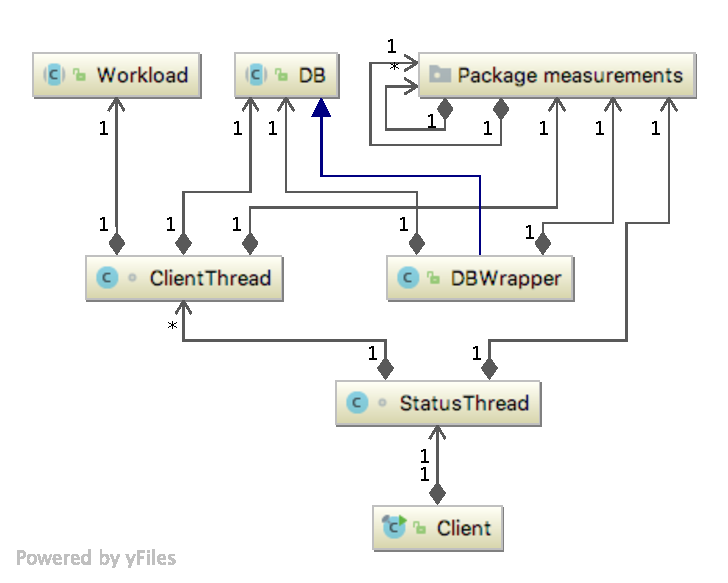
\includegraphics[width=.75\textwidth]{images/benchmarks/basicYCSBWorkflow}
  \caption{Class diagram of the main classes involved in YCSB.}
  \label{fig:basicYCSBWorkflow}
\end{figure}

The workload file specifies some parameters of the workload.
These are among others,
the workload class to use,
how much data should be added in the load phase,
how much operations should be executed in the transaction phase and what percentage of the operations should be inserts, reads, updates, scans or deletes.

The measurements can be saved as histograms each covering one particular operation.
There is also a summary printed out to the console or a file depending on the parameters you set that additionally lists the overall time for the benchmark, times of the individual operations and some more meta information.
     % Analyse
\chapter{Design}
\label{ch:design}

In this chapter we will design the data structure of our test data,
as well as the workloads to simulate a typical industrial use of our examined databases.

After that we will plan our extension for YCSB in section~\ref{ch:design:se:extensionOfTheBenchmark},
both for the internals of the benchmark and the bindings to connect the databases.

In the end in section~\ref{ch:design:se:executionTool} and~\ref{ch:design:se:evaluationTool} we will outline tools to support execution of the benchmark and evaluation of the results.

\section{Data Structure}
\label{ch:design:se:dataStructure}
To create a schema for our data structure we had a meeting with other researchers at our institute.
The result of our session can be seen in figure~\ref{fig:firstDesignOfSchema}.
In the centre left we see "Features of Interest" which could be mapped to the "testFeature" edge in the industrial example of figure~\ref{fig:exampleData} as it depicts an observation of some product.
At the bottom we see a "M" which stands for "Machine",
its connection to "P. Schritte"\footnote{german for production steps} shows that this machine does \texttt{1} to \texttt{n} production steps.
Every production step is associated with a component which consists of a PCB\footnote{short for printed circuit board} that has different parts,
a version and a file after which it was created.

As the model shows too much detail in some areas without giving a good overview of an industrial data schema,
we had to reiterate over it and get rid of some complexity where we don't need it for our purposes.

\begin{figure}
  \centering
  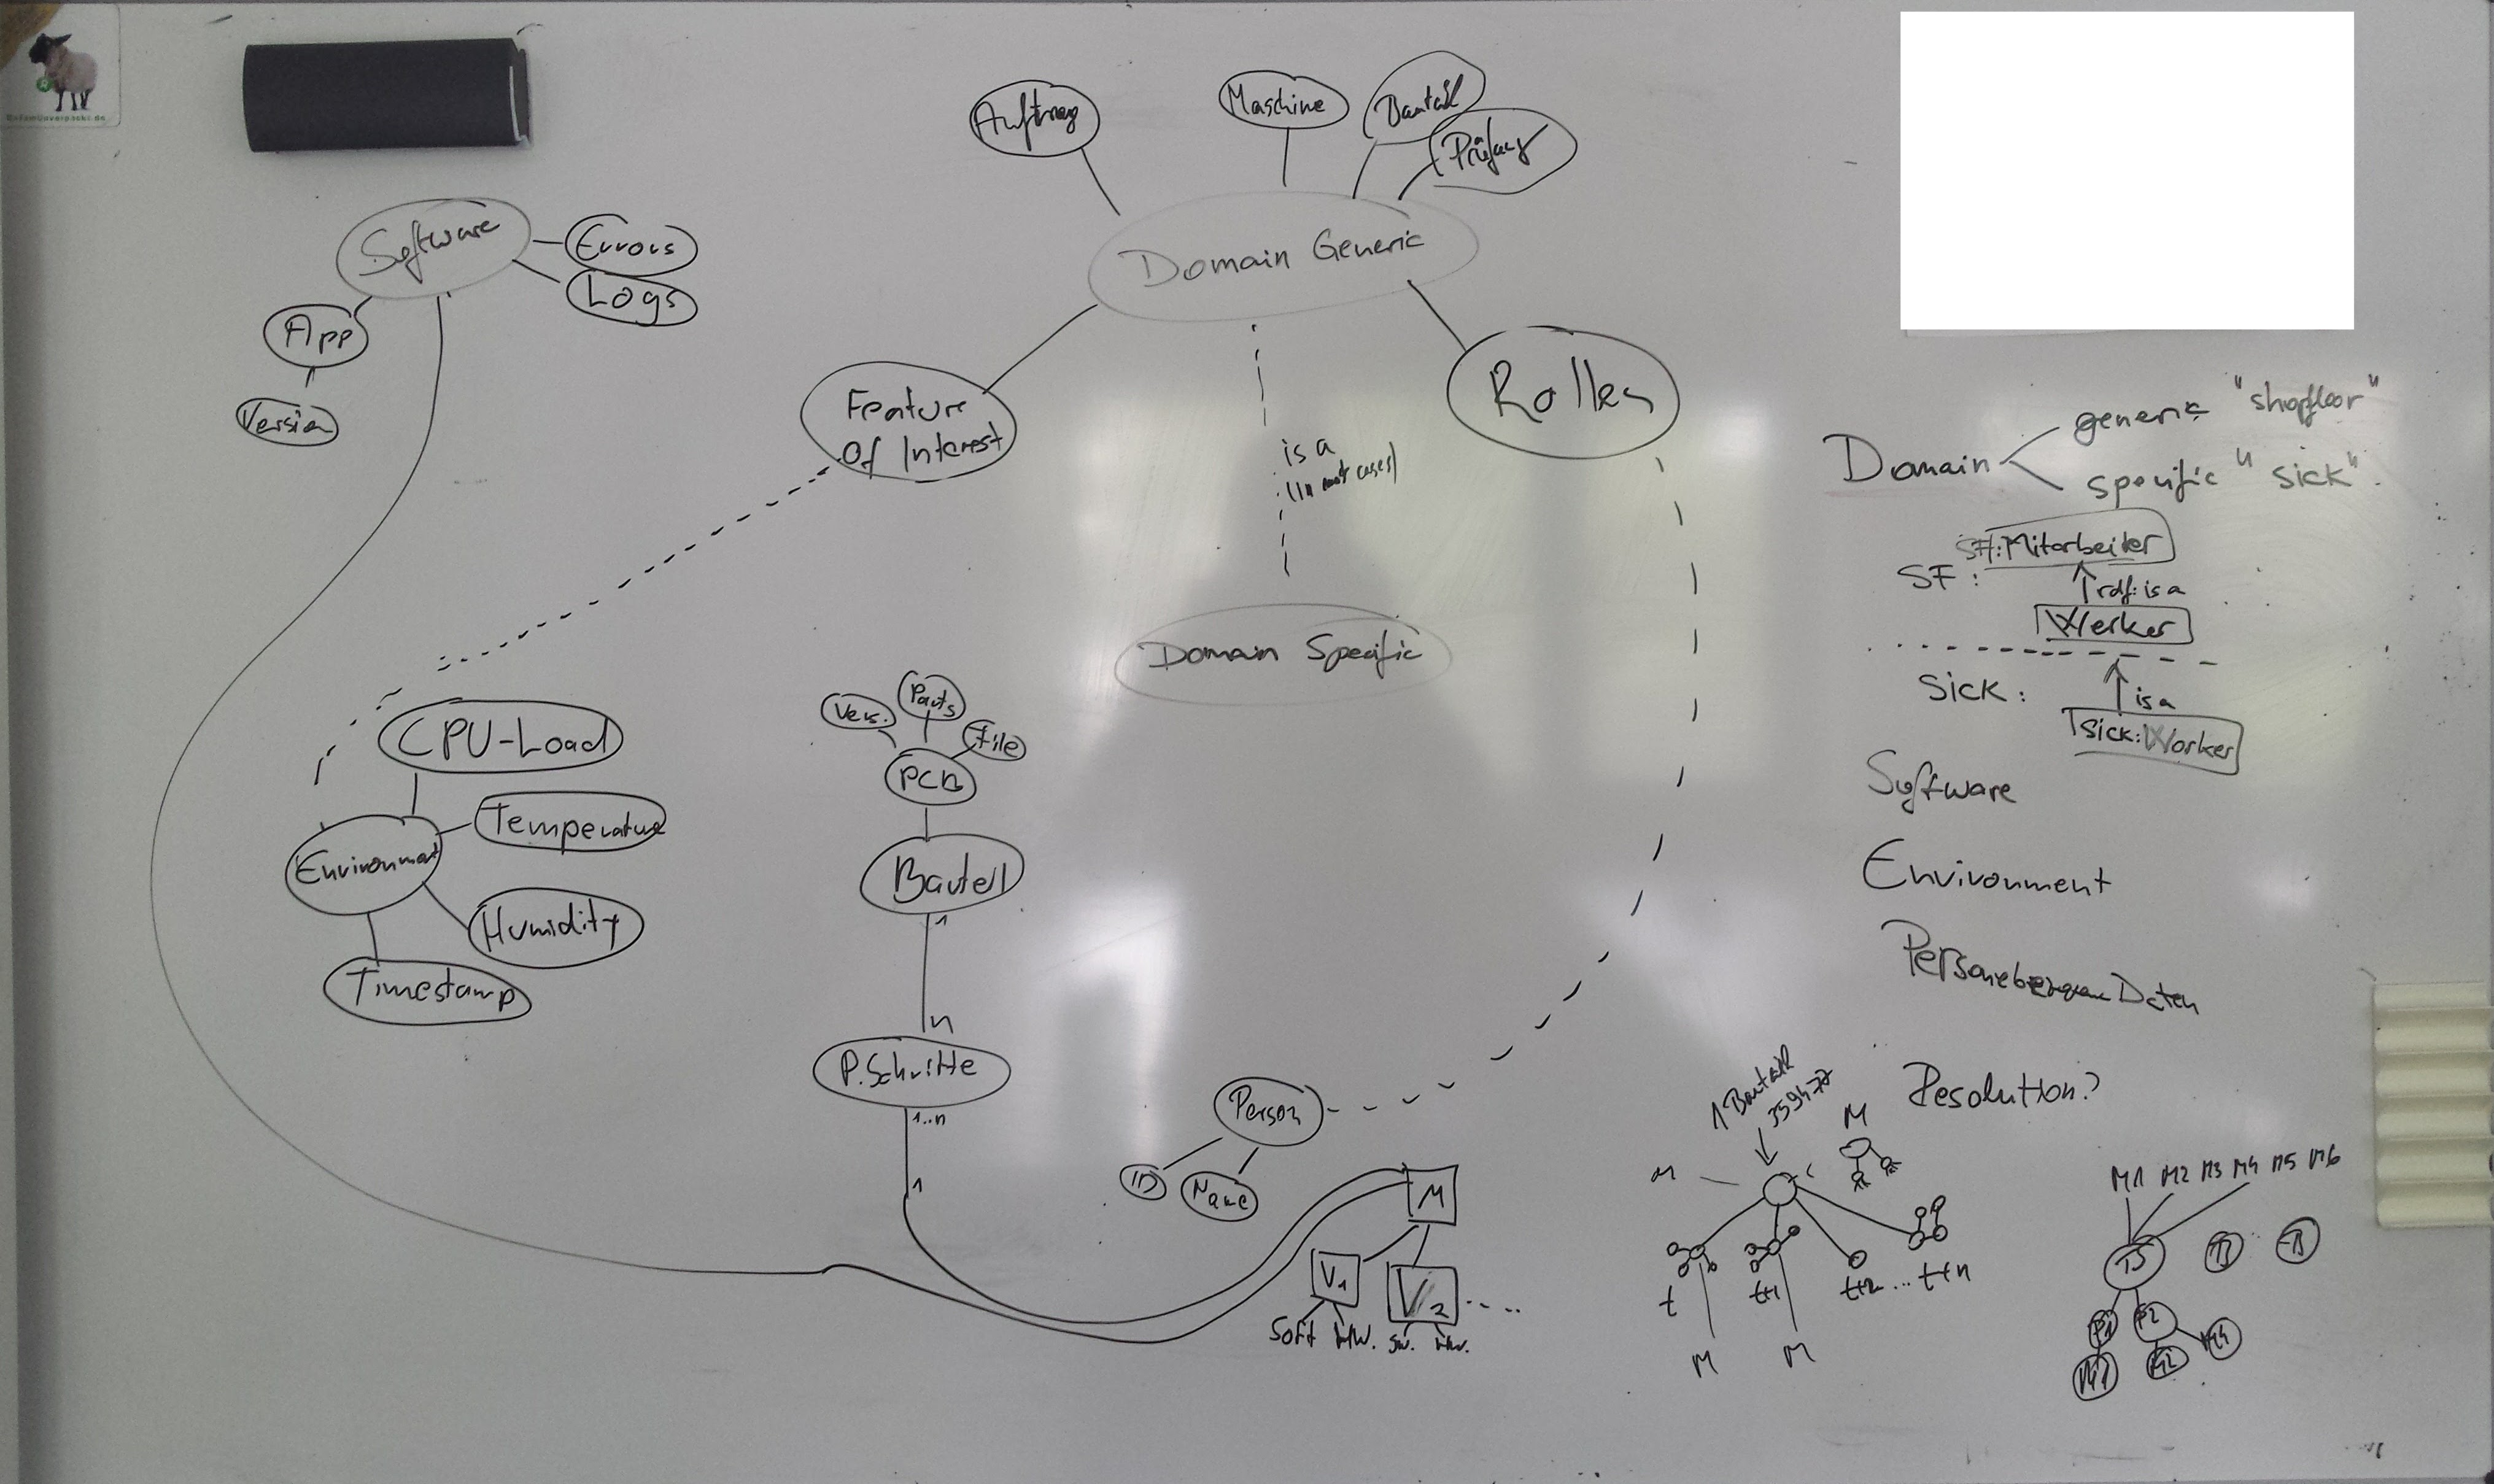
\includegraphics[width=\textwidth]{images/design/firstDesignOfSchema}
  \caption{The first design of a data schema for industrial data. Created by researchers at our institute.}
  \label{fig:firstDesignOfSchema}
\end{figure}

The meeting gave us a better understanding of how a production facility could handle its data and with that in mind and the objective to design a simpler schema that includes to most necessary parts of production the model shown in figure~\ref{fig:finalDesignOfSchema} was created. \\
At the top is the \texttt{Factory},
which has an \texttt{Orders} node that represents the folder for all \texttt{Order}s received by the \texttt{Factory}.
A \texttt{Machine} and a \texttt{Design} are linked to the \texttt{Factory},
these represent the production machine and the design template for products made by that machine.
A \texttt{Product} has incoming edges from the \texttt{Design} it is made after, the \texttt{Machine} it was produced by and the \texttt{Order} for which it is created.
Variable x determines how many \texttt{Product}s are made for each \texttt{Order}.
The \texttt{Product} was made at a specific \texttt{Date} and consists of one or multiple \texttt{Component}s depending on the value of variable y.
Every \texttt{Component} undergoes a test suite (\texttt{Tests}) which contains of a number of \texttt{Test Parameter}s,
which number is defined by z.\\
For easier reference we will call x productsPerOrder, y componentsPerProduct and z testParameterCount.

\begin{figure}
  \centering
  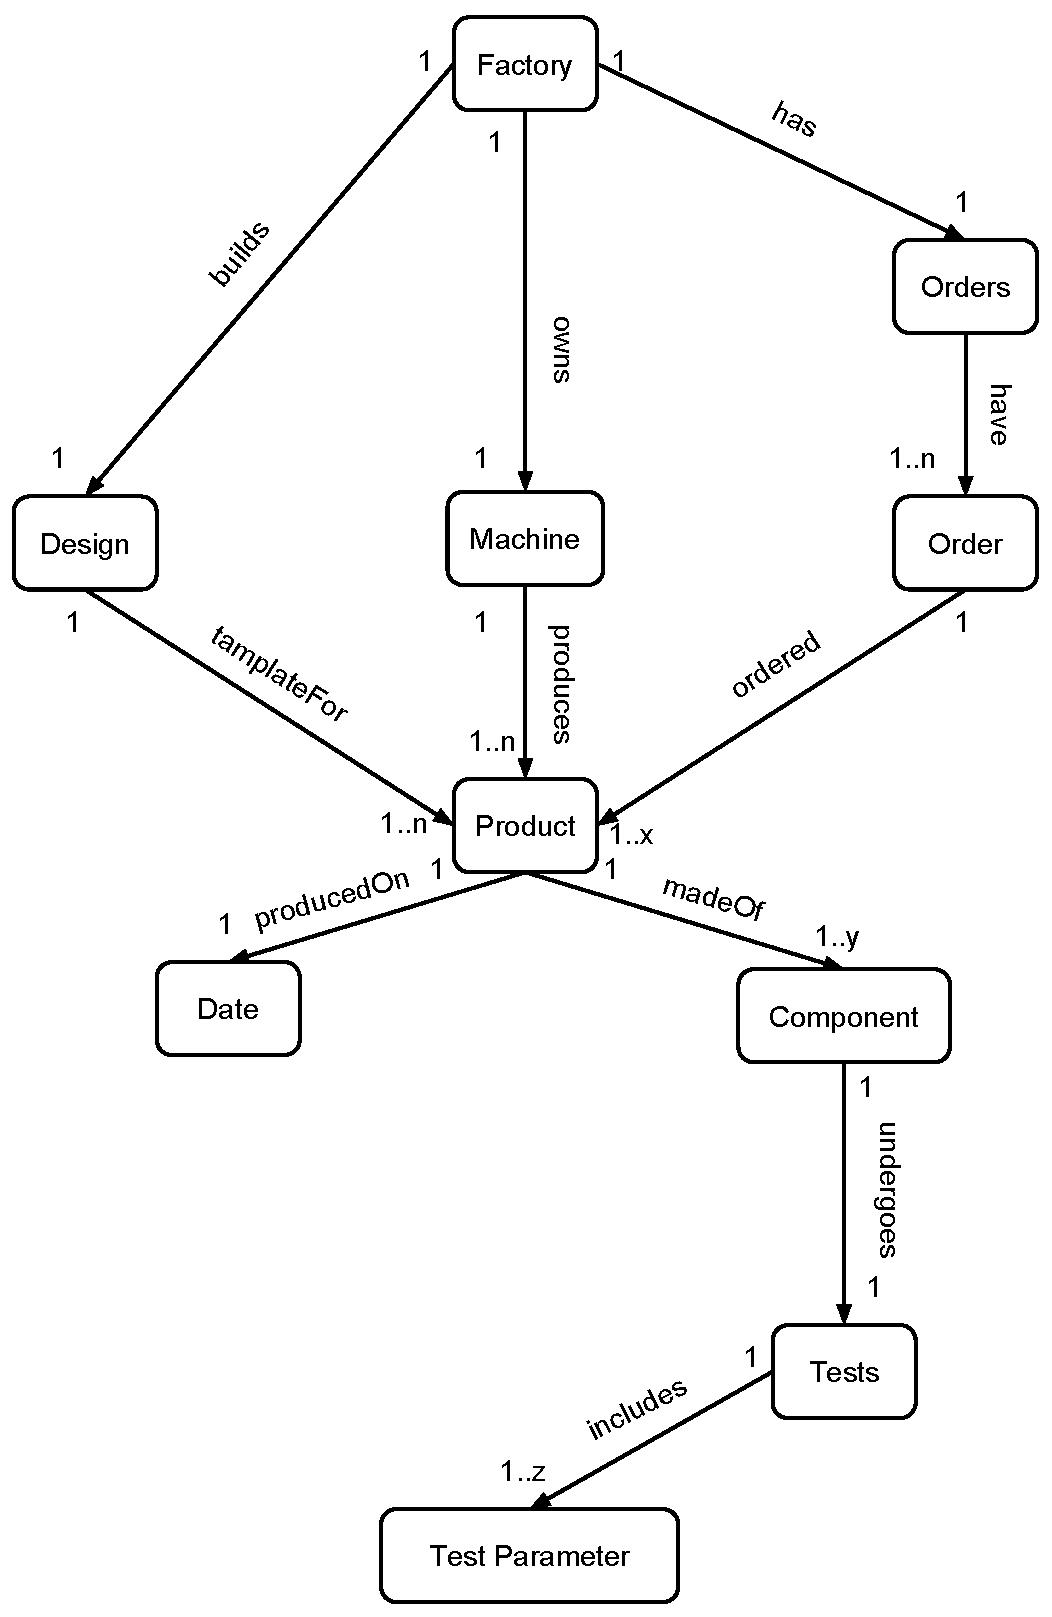
\includegraphics[width=.75\textwidth]{images/design/dataStructure}
  \caption{The final design of the data schema.}
  \label{fig:finalDesignOfSchema}
\end{figure}

\section{Workloads}
\label{ch:design:se:workloads}
Our workload design will be separated into three parts.
In subsection~\ref{ch:design:se:throughput} we discuss the design of workloads aimed to uncover the ability to store large amounts of data.
Subsection~\ref{ch:design:se:productionSimulation} will directly investigate the suitability of a database to be used in an industrial use case for storing data.
We will design workloads to examine the other industrial use case of retrieving data under load in subsection~\ref{ch:design:se:retrievingUnderLoad}.
Finally we will give a summary over all workloads we are going to run on the databases in subsection~\ref{ch:design:se:summary}

\subsection{Throughput}
\label{ch:design:se:throughput}
To explore the throughput of the databases we will have some variables we will change over the course of the different workloads.
These variables are

\begin{itemize}
  \item using an index on the key
  \item the size of a single property of the node
  \item using no edges with and without an index.
\end{itemize}

The last variable sounds counter intuitive,
since edges add meaning to the data,
but by eliminating them we want to see if edges could be a cause of delay,
because to add an edge the start and end node need to be known and therefore be retrieved at first.

We will go over the different variables in the following subsections and motivate their purpose.

\subsubsection{Index}
\label{ch:design:se:index}
For this category we will use different data set sizes in terms of their number of nodes.
We will use steps of multiplication by 10 from 1.000 nodes to 10.000.000 nodes,
to examine if the throughput changes,
as the database is filled with data.

Switching from indexed to not indexed we want to inspect how the throughput is effected by not using an index.
Indexing is important to retrieve data more quickly for the cost of write speed,
with this workload we will see if there is a sacrifice in write throughput,
as to store an edge,
two nodes have to be looked up.
We will only use an index on the node and edge key,
which will be used to search that graph component\footnote{a node or an edge of the graph} in the database.
Indexing the other properties would have no benefit in our example.

For this workload we will use a node property size of 10B,
that is small enough to not have an impact on performance but large enough to represent most of the data stored in the properties of our example.

\subsubsection{Node Property Size}
\label{ch:design:se:nodePropertySize}
After retrieving a number of nodes that represents an acceptable execution time we will vary the next variable which is the property size.
We will go from 10B used in the index benchmarks to up to 1MB,
again in steps of multiplying by 10 (10B, 100B, 1KB, ..., 1MB).
We want to examine if there is a drawback for throughput when storing more information in the nodes and at which point the amount is too large.

The typical property size is between 1B (1 character) and roughly 75B (75 characters) according to our example in listing~\ref{lst:exampleData}.

The use of properties is not limited to short strings,
that is why we will investigate if larger amounts of data influence the throughput more than linearly.

We will use an index on the keys,
because using an index would represent the use in the industry and since we are not indexing the growing values there will be no impact from using it.

\subsubsection{No Edges}
\label{ch:design:se:noEdges}
In subsection~\ref{ch:design:se:throughput} we already justified why we will investigate the throughput with an exclusive use of nodes in the data set.
To summarise the use of this workload is to see if there is a big difference in using edges and therefore determine how the edge to node ratio effects the throughput.

As in subsection~\ref{ch:design:se:nodePropertySize} we will use a suitable large data set in terms of node count resulting from the first workloads.
We will use the same node size as in~\ref{ch:design:se:index} and an index to be able to compare the results directly to the corresponding ones from that workload.

\subsection{Production Simulation}
\label{ch:design:se:productionSimulation}
Related to production we will investigate the impact of the structure and the general suitability for an industrial use.
The next two subsections will cover those aspects in more detail.

The property size will be set to 50B,
which should be enough to cover on average most values stored in the database.

\subsubsection{Structure}
For production we have some variables to investigate which mainly effect the structure of our data.
We have three layers which we can blow up horizontally by increasing the corresponding parameters,
which are

\begin{itemize}
  \item productsPerOrder, this spreads the data graph apart at a level closer to the root
  \item componentsPerProduct, this changed the width in the middle of the graph
  \item testParameterCount, which widens the graph at the lowest level.
\end{itemize}

For production simulation we will first examine if the data structure impacts performance of the databases.
To investigate this aspect,
we will change the width of the graph with the variables mentioned above.
We will use the numbers from section~\ref{ch:analysis:se:data} as the maximum width,
which would be \texttt{productsPerOrder = 64},
\texttt{componentsPerProduct = 128} and \texttt{testParameterCount = 128}.
In the first workload we will set all variables to one,
the next one will use \texttt{productsPerOrder = 16},
\texttt{componentsPerProduct = 32} and \texttt{testParameterCount = 32}.
The third and last one will use the maximum width mentioned above.
By this variation we will cover the minimum and maximum with an additional result in the middle to see if there are any changes in performance.

The keys of the graph components will be indexed,
because indexing these values should be done to later work on that data more efficiently,
which is necessary for the industry.

\subsubsection{Suitability}
\label{ch:design:se:suitability}
To examine if a database is suitable for the industry it should be able to store the data faster than it is coming from the machines.
In section~\ref{ch:analysis:se:dataAmount} we calculated that 1056833 nodes would be written to the database every three minutes.

Now that we have our data structure we can calculate how many edges are contained in that graph and finally how many inserts have to be performed every second.
We will count the incoming edges for every node and also use the variables x, y and z from the structure in~\ref{ch:design:se:dataStructure}.

\begin{equation}
  \label{eq:dataEdges}
  \begin{aligned}
    n_{edges} &= n_{Design} + n_{Machine} + n_{Orders} + n_{Order} + 3 \times n_{Product} \\
    &\quad + n_{Product} \times (n_{Date} + n_{Component} \times (n_{Tests} + n_{TestParameter})) \\
    \iff &= 1 + 1 + 1 + 1 + 3 \times x + x \times (1 + y \times (1 + z)) \\
    \iff &= 4 + 3 \times x + x \times (1 + y \times (1 + z)) \quad | x = 64, y = 128, z = 128 \\
    \implies &= 4 + 3 \times 64 + 64 \times (1 + 128 \times (1 + 128)) \\
    \iff &= 4 + 192 + 64 \times (1 + 128 \times 129) \\
    \iff &= 4 + 192 + 64 \times (1 + 16512) \\
    \iff &= 4 + 192 + 64 \times 16513 \\
    \iff &= 4 + 192 + 1056832 \\
    \iff &= 1057028
  \end{aligned}
\end{equation}

Together with the number of nodes we can calculate the total amount of elements being inserted into the database as shown in equation~\ref{eq:dataElements}.

\begin{equation}
  \label{eq:dataElements}
  \begin{aligned}
    n_{total} &= n_{nodes} + n_{edges} \\
    \iff &= 1056833 + 1057028 \\
    \iff &= 2113861
  \end{aligned}
\end{equation}

To convert that into our target throughput we divide that number by three minutes.

\begin{equation}
  \label{eq:dataElements}
  \begin{aligned}
    n_{target} &= n_{total} \times \frac{1}{3 \times 60s} \\
    \iff &= 2113861 \times \frac{1}{180s} \\
    \iff &= 11743,67 \frac{1}{s}
  \end{aligned}
\end{equation}

First,
we will set up a data set with that number of nodes and insert it into the database,
that will allow us to compare the time needed to store all data with our three-minute limit.
If the database should take more than three minutes,
it would not be suitable,
since data is produced faster than it can be stored.

We will use the structure with the maximum width,
because it represents the industrial use case the best regarding the information given by our partners at SICK AG~\cite{SICK}.

\subsection{Retrieving under load}
\label{ch:design:se:retrievingUnderLoad}
There would be no point in storing data if it is not retrieved at some point.
To investigate on the performance of reading and scanning (more on that in subsection~\ref{ch:design:se:scanning}) data from the database the following workloads are designed.

As mentioned in section~\ref{ch:design:se:index} indexing is important for retrieving data,
therefore we will use it as a variable for this workload category.
By doing so we want to examine if the price we pay while writing is justified by the performance gain in retrieving data.

The node amount will be determined by the first workload investigating the throughput,
to not take up too much time testing these features.

We want to retrieve both nodes and edges,
because either could be useful,
since the edges can also store properties in them.

\subsubsection{Reading}
\label{ch:design:se:reading}
Reading single values is the basic operation when it comes to retrieving data from a database.
Since the database will be under constant load,
because of production delivering data all the time,
we will use $ 5\% $ of the total operations executed in this workload for read operations,
the rest will be inserting data.

\subsubsection{Scanning}
\label{ch:design:se:scanning}
Scanning a graph can be done in multiple ways,
the simplest being depth first search~\cite{Tarjan1972},
to retrieve values associated with connected nodes.
For example,
you could scan from a machine to get the test features of their produced products.

As in subsection~\ref{ch:design:se:reading} we will use a mix of $ 5\% $ scan operations with $ 95\% $ insert operations,
to simulate the constant load present in an industrial environment.

The number of steps to do during scanning will be $ 1000 $ as that was the default value set in YCSB and it should also represent a good amount of data to read.

\subsection{Summary}
\label{ch:design:se:summary}
In this subsection we will give an overview over all workloads and their variables.

For the workloads measuring the throughput \texttt{productsPerOrder},
\texttt{componentsPerProduct} and \texttt{testParameterCount} will all be set to $ 1 $.
Their overview is shown in table~\ref{tab:throughput}

\begin{table}[!h]
  \begin{minipage}{\textwidth}
    \begin{tabularx}{\textwidth}{ | X | X | X | X | X | }
      \hline
      Aspect & Node Count & Node Size & Index & Only Nodes \\ \hline
      1. With Index & 1.000 & 10B & True & False \\ \hline
      2. With Index & 10.000 & 10B & True & False \\ \hline
      3. With Index & 100.000 & 10B & True & False \\ \hline
      4. With Index & 1.000.000 & 10B & True & False \\ \hline
      5. With Index & 10.000.000 & 10B & True & False \\ \hline
      1. Without Index & 1.000 & 10B & False & False \\ \hline
      2. Without Index & 10.000 & 10B & False & False \\ \hline
      3. Without Index & 100.000 & 10B & False & False \\ \hline
      4. Without Index & 1.000.000 & 10B & False & False \\ \hline
      5. Without Index & 10.000.000 & 10B & False & False \\ \hline
      1. Node Size & x & 100B & True & False \\ \hline
      2. Node Size & x & 1KB & True & False \\ \hline
      3. Node Size & x & 10KB & True & False \\ \hline
      4. Node Size & x & 100KB & True & False \\ \hline
      5. Node Size & x & 1MB & True & False \\ \hline
      1. No Edges & x & 10B & True & True \\ \hline
    \end{tabularx}
  \end{minipage}
  \caption{Workloads to investigate the throughput. x is a placeholder for a suitable data set size in terms of execution time.}
  \label{tab:throughput}
\end{table}

The workloads to investigate the suitability for the industry are shown in table~\ref{tab:productionSimulation}.
For these workloads the property size is fixed to 50B and an index is used on all workloads.
Edges are also used in these workloads to reflect the use in the industry.

\begin{table}[!h]
  \begin{minipage}{\textwidth}
    \begin{tabularx}{\textwidth}{ | X | X | X | X | X | }
      \hline
      Aspect & Node Count & products\-Per\-Order & components\-Per\-Product & test\-Parameter\-Count \\ \hline
      1. Structure & x & 1 & 1 & 1 \\ \hline
      2. Structure & x & 16 & 32 & 32 \\ \hline
      3. Structure & x & 64 & 128 & 128 \\ \hline
      1. Suitability (three minutes) & 1.056.833 & 64 & 128 & 128 \\ \hline
      2. Suitability (hour) & 21.136.660 & 64 & 128 & 128 \\ \hline
      3. Suitability (day) & 507.279.840 & 64 & 128 & 128 \\ \hline
      4. Suitability (week) & 3.550.958.880 & 64 & 128 & 128 \\ \hline
      5. Suitability (month) & 15.218.395.200 & 64 & 128 & 128 \\ \hline
      6. Suitability (year) & 185.157.141.600 & 64 & 128 & 128 \\ \hline
    \end{tabularx}
  \end{minipage}
  \caption{Workloads to simulate production. Again, x represents a placeholder for a suitable data set size.}
  \label{tab:productionSimulation}
\end{table}

The remaining workloads to examine the ability to retrieve data are shown in table~\ref{tab:retrievingUnderLoad}.
These workloads will use an appropriate data set size regarding execution time and a property size as in the production simulation of 50B.
A simple structure is used to investigate the basic capabilities of data retrieval,
that means \texttt{productsPerOrder},
\texttt{componentsPerProduct} and \texttt{testParameterCount} are set to $ 1 $.

\begin{table}[!h]
  \begin{minipage}{\textwidth}
    \begin{tabularx}{\textwidth}{ | X | X | X | X | X | }
      \hline
      Aspect & Index & Insert Proportion & Read Proportion & Scan Proportion \\ \hline
      1. Reading & True & 95\% & 5\% & 0\% \\ \hline
      2. Reading & False & 95\% & 5\% & 0\% \\ \hline
      1. Scanning & True & 95\% & 0\% & 5\% \\ \hline
      2. Scanning & False & 95\% & 0\% & 5\% \\ \hline
    \end{tabularx}
  \end{minipage}
  \caption{Workloads to investigate capability to retrieve data under load.}
  \label{tab:retrievingUnderLoad}
\end{table}

\section{Extension of the Benchmark}
\label{ch:design:se:extensionOfTheBenchmark}
To be able to execute the introduced workloads and use the data structure designed above,
we need to extend the YCSB benchmark.
For the benchmark to be able to execute our workloads the way we want them to be executed the following parts of the benchmark need to be extended

\begin{itemize}
  \item Generation of the dataset
  \item Generation of random graph components
  \item Generation of an operation order
  \item Workload to use the generated dataset
  \item Database bindings.
\end{itemize}

In the following subsections we will go in more detail over the different areas we are planning to modify.

\subsection{Graph Data Generator}
YCSB does not include a graph data generator,
therefore we need to create one that fulfils our needs.

The generator should create a data set with the structure mentioned in section~\ref{ch:design:se:dataStructure} and store the data for future reproduction when using the benchmark with the next database.

The two parts of the generator,
which are creating together with storing the data and recreating the data are designed in subsection~\ref{ch:design:se:storingTheDataset} and~\ref{ch:design:se:restoringTheDataset} respectively.

Generally,
to represent a graph in YCSB we need some classes to represent nodes, edges and the graph.
In section~\ref{ch:background:se:graphs} we mentioned that a graph is a tuple of a set of nodes and a set of edges.
That can be directly mapped to a class with two lists,
one for nodes and the other one for edges.
We want the nodes to have a key for identification,
a label to match it with an object that could exist in the real world and a value,
which will represent the data stored in the node,
the size of this value should be directly linked to the property size from~\ref{ch:design:se:nodePropertySize}.
An edge should also have a key for identification,
a label to add meaning to it and a start and an end node,
represented by their keys.

The generator of the dataset should decide if it should create a new one or recreate it by looking at the existing files.

\subsubsection{Storing the Dataset}
\label{ch:design:se:storingTheDataset}
We want to control the size of the dataset with our variables mentioned in the workload section~\ref{ch:design:se:workloads} so this generator should create small subgraphs with only one node and its corresponding edges every time it is asked for a new value.
By storing the current state of the created graph in the generator class,
we can always determine the next subgraph to create.

The modify the structure of the graph with our three variables,
these need to be parsed in this class and used during subgraph creation.

To restore that data also one node at a time we will store each created subgraph in a file,
for that we will serialise the graph and deserialise it when we are restoring the data.

To disable edges for the workload from subsection~\ref{ch:design:se:noEdges} we can simply skip the step of creating and adding them to the graph.

\subsubsection{Restoring the Dataset}
\label{ch:design:se:restoringTheDataset}
The restoring of the data should be easily done by deserialising it from the created file during creation of the dataset.
Since the single subgraphs were stored in the file,
we can pass the to the workload just after deserialising them.

For larger datasets we should read the subgraphs from the file as needed and not at the beginning,
because that could fill up the RAM with the dataset and leave less memory for the database to work with.

\subsection{Random Graph Component Generator}
Reading and scanning operations require a point to start with in the data,
that's why we need the key of some component in the graph.
The kay can be randomly chosen,
but the node or edge associated with it has to be present in the database.
Therefore,
we need to somehow store the keys of the graph components we have already put into the database,
that could be done in the \texttt{GraphDataGenerator} created for subsection~\ref{ch:design:se:storingTheDataset},
because it anyway touches all created values.

Because we want to retrieve edges and nodes randomly we have to pick one of the two randomly every time a random component is required.
As in~\ref{ch:design:se:storingTheDataset} and its subsections,
every created value needs to be stored to be retrieved later on.
The data needed for this generator is not as complex as a graph and can therefore be stored directly in a file line by line for easy storing and restoring.
That also means,
that we can read the files at the beginning of the run so it is faster accessible during the benchmark without using too much memory.

For the workload which requires the absents of edges a method should be defined to return only a randomly chosen node.

Figure~\ref{fig:randomGraphComponentGenerator} shows an activity diagram of the generator returning a random graph component.

\begin{figure}
  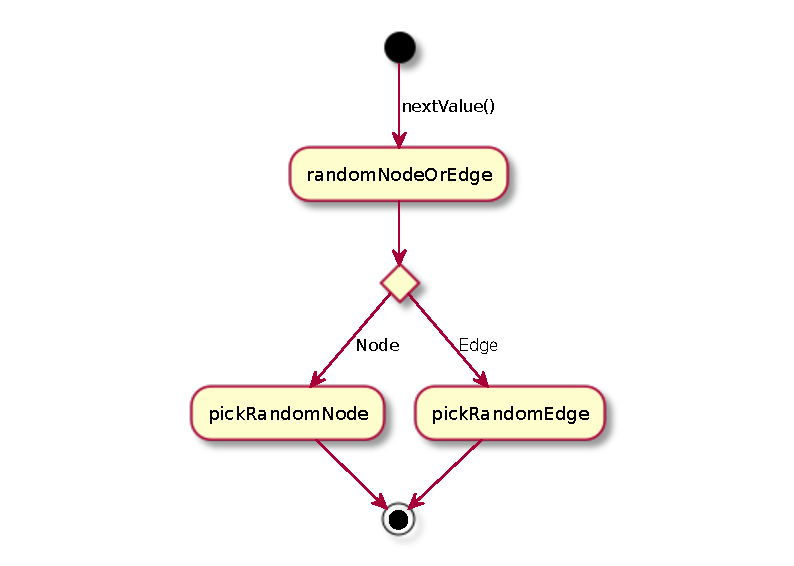
\includegraphics[width=\textwidth]{images/extensions/randomGraphComponentGenerator}
  \caption{Activity diagram of the \texttt{RandomGraphComponentGenerator} showing the process of storing and restoring.}
  \label{fig:randomGraphComponentGenerator}
\end{figure}

\subsection{Operation Order Generator}
\label{ch:design:se:operationOrderGenerator}
To fix the execution order of inserting and retrieving data to and from the graph,
we need to store the operations too.
That can be done by simply storing the name of each operation in a file as it appears and reading it from there when running the benchmark.

In YCSB there is already a \texttt{DiscreteGenerator}\footnote{com.yahoo.ycsb.generator.DiscreteGenerator} which take a value and a weight and returns distributed according to the weights a value,
this can be used to get the operations to run on the database.

Figure~\ref{fig:operationOrderGenerator} visualises the procedure to return the next operations.

\begin{figure}
  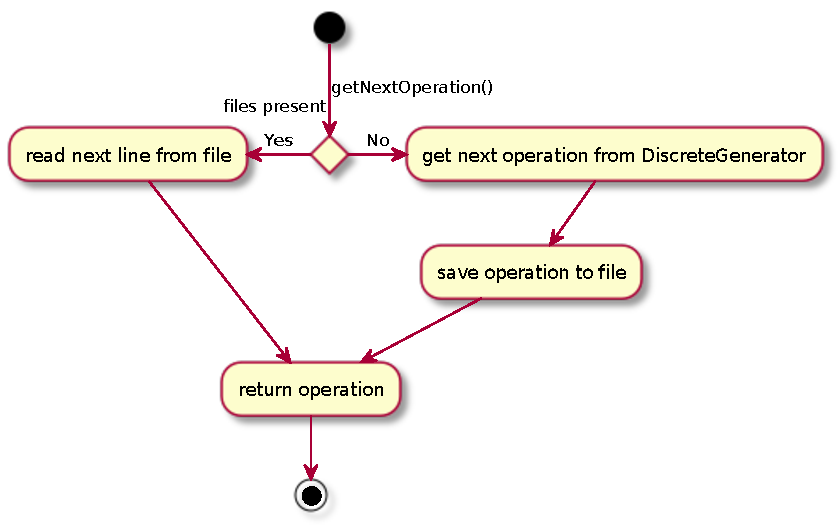
\includegraphics[width=\textwidth]{images/extensions/OperationOrderGenerator}
  \caption{Activity diagram of the operationOrderGenerator.}
  \label{fig:operationOrderGenerator}
\end{figure}

\subsection{Graph Workload}
The \texttt{GraphWorkloads} task is to coordinate the different generators and to execute the workload as specified.
To be able to store the generated dataset in a specific folder on the system the workload class should take a path to a folder and instrument the generators to store their data in that folder or recreate it from there respectively.

This class will be the interface between the client calling \texttt{Workload::doInsert} and \texttt{Workload::doTransaction} and the database.
The \texttt{Workload::doInsert} method will only insert a subgraph into the database,
to do so the workload class needs to get the subgraph from the GraphDataGenerator and redirect its value to the database.
For the \texttt{Workload::doTransaction} method the workload has to be able to call the available methods on a database which are

\begin{itemize}
  \item DB::insert(String table, String key, Map<String, ByteIterator> values)
  \item DB::read(String table, String key, Set<String> fields, Map<String, ByteIterator> result)
  \item DB::scan(String table, String key, int recordcount, Set<String> fields, Vector<HashMap<String, ByteIterator>{}> result)
  \item DB::update(String table, String key, Map<String, ByteIterator> values)
  \item DB::delete(String table, String key).
\end{itemize}

We will only use the first three for our workloads,
but the other ones should be implemented too,
to support future workloads.
To determine which operation should be executed the \texttt{OperationOrderGenerator} from subsection~\ref{ch:design:se:operationOrderGenerator} will be used.

In general,
we see that a \texttt{table} is given as an argument,
in a graph database we don't have tables as in relational databases,
so we can use it to distinguish between nodes and edges,
by simply passing the string "node" or "edge" to the database.
Next is a \texttt{key},
which we can use to pass the key identifier of the graph component to the database.
The \texttt{values} map will contain the values of the graph components to insert parsed into a map for compatibility and vice versa for the \texttt{result} map and vector.
Our data design does not focus to much on the individual properties the nodes and edges could have,
therefore we will simply read all \texttt{fields} of the graph component.

\textbf{DB::insert} \newline
As described above the \texttt{DB::insert} method will get a value from the \texttt{GraphDataGenerator} and insert it into the database.

\textbf{DB::read} \newline
The read operation will pick a random graph component with the \texttt{RandomGraphComponentGenerator} and use its kind (node or edge) as the \texttt{table} argument and the key identifier as the \texttt{key} argument.

\textbf{DB::scan} \newline
Scanning also requires a random component which will be chosen by the \texttt{RandomGraphComponentGenerator}.
The mapping is also the same as with \texttt{DB::read} for the \texttt{table} and \texttt{key} arguments.
\texttt{recordcount} will be set to $ 1000 $ as that is the default value specified by the \texttt{CoreWorkload}\footnote{com.yahoo.ycsb.workloads.CoreWorkload} and that value represents a good amount for scanning.

\textbf{DB::update} \newline
For this operation we need a randomly picked graph component from the \texttt{RandomGraphComponentGenerator} to get a valid key identifier.
Only the property value should be changed during update,
not the identifier nor the label,
that means that only nodes will be changes,
as edges have no property value assigned to them.

\textbf{DB::delete} \newline
This takes a random graph component via the \texttt{RandomGraphComponentGenerator} and calls the \texttt{delete} method of the database.

To avoid calling these methods with edges when the workload specifies to not use them,
a parameter which can be set should determine if a random graph component or a random node should be picked by the \texttt{RandomGraphComponentGenerator}.

Since the client only calls \texttt{Workload::doTransaction} to execute one of the various database operations the \texttt{OperationOrderGenerator} should be called to generate the next operation.

\subsection{Bindings}
\label{ch:design:se:bindings}
To ensure compatibility with other workloads present in YCSB we will extend the \texttt{DB} class and implement the methods used for other databases.
Because graph databases are slightly different we will explain how each database will map the arguments of the \texttt{DB} methods to their own API in the following subsections.

The basic functions we need from our database are

\begin{enumerate}
  \item creating a node
  \item creating an edge
  \item adding properties to a node
  \item adding properties to an edge
  \item getting a node by its identifier
  \item getting an edge by its identifier
  \item getting the values of a node
  \item getting the values of an edge
  \item getting the outgoing edges of a node
  \item getting the start node of an edge
  \item removing a node
  \item removing an edge
\end{enumerate}

Generally,
the \texttt{DB} operations can then be implemented using these functions.
A rough implementation is shown in listing~\ref{lst:databaseTemplate}.
Every database will take a path to a folder in which it will store its internally used files.
Also,
if indexing is possible every database should take it as a parameter to set itself up correctly.

We will cover the implementation of the single methods in section~\ref{ch:implementation:se:graphDatabaseBindings}.
The following subsections will only mention specialities regarding the corresponding database.

\begin{lstlisting}[language={Java},label={lst:databaseTemplate},caption={Generic example of a database implementation with the use of graph data.},captionpos=b]
public class Database extends DB {
  private Node creatingANode(String key);
  private Edge creatingAnEdge(String key, Node startNode, Node endNode);
  private void addingPropertiesToANode(Node node, Map<String, ByteIterator> values);
  private void addingPropertiesToAnEdge(Edge edge, Map<String, ByteIterator> values);
  private Node gettingANodeByItsIdentifier(String key);
  private Edge gettingAnEdgeByItsIdentifier(String key);
  private HashMap<String, ByteIterator> gettingTheValuesOfANode(Node node);
  private HashMap<String, ByteIterator> gettingTheValuesOfAnEdge(Edge edge);
  private List<Edge> gettingTheOutgoingEdgesOfANode(Node node);
  private Node gettingTheStartNodeOfAnEdge(Edge edge);
  private void removingANode(String key);
  private void removingAnEdge(String key);

  private void doDepthFirstSearchOnNodes(Node node, int recordcount, Vector<HashMap<String, ByteIterator>> result) {
    if (result.size() >= recordcount) {
      return;
    }

    result.add(gettingTheValuesOfANode(node));

    List<Edge> edges = gettingTheOutgoingEdgesOfANode(node);

    for (Edge edge : edges) {
      Node startNode = gettingTheStartNodeOfAnEdge(edge);
      doDepthFirstSearchOnNodes(startNode, recordcount, result);
    }
  }

  private void doDepthFirstSearchOnEdges(Node node, int recordcount, Vector<HashMap<String, ByteIterator>> result) {
    if (result.size() >= recordcount) {
      return;
    }

    List<Edge> edges = gettingTheOutgoingEdgesOfANode(node);

    for (Edge edge : edges) {
      result.add(gettingTheValuesOfAnEdge(edge));

      Node startNode = gettingTheStartNodeOfAnEdge(edge);
      doDepthFirstSearchOnNodes(startNode, recordcount, result);
    }
  }

  @Override
  public Status insert(String table, String key, Map<String, ByteIterator> values) {
    switch(table) {
    case "Node":
      Node node = creatingANode(key);
      addingPropertiesToANode(node, values);
      break;
    case "Edge":
      Node startNode = gettingANodeByItsIdentifier(values.get("startNode").toString());
      Node endNode = gettingANodeByItsIdentifier(values.get("endNode").toString());
      Edge edge = creatingAnEdge(key, startNode, endNode);
      addingPropertiesToAnEdge(edge, values);
      break;
    default:
      return Status.NOT_FOUND;
    }
    return Status.OK;
  }

  @Override
  public Status read(String table, String key, Set<String> fields, Map<String, ByteIterator> result) {
    switch(table) {
    case "Node":
      Node node = gettingANodeByItsIdentifier(key);
      result = gettingTheValuesOfANode(node);
      break;
    case "Edge":
      Edge edge = gettingAnEdgeByItsIdentifier(key);
      result = gettingTheValuesOfAnEdge(edge);
      break;
    default:
      return Status.NOT_FOUND;
    }
    return Status.OK;
  }

  @Override
  public Status scan(String table, String startkey, int recordcount, Set<String> fields, Vector<HashMap<String, ByteIterator>> result) {
    switch(table) {
    case "Node":
      Node node = gettingANodeByItsIdentifier(startkey);
      doDepthFirstSearchOnNodes(node, recordcount, result);
      break;
    case "Edge":
      Edge edge = gettingAnEdgeByItsIdentifier(startkey);
      Node startNode = gettingTheStartNodeOfAnEdge(edge);
      doDepthFirstSearchOnEdges(startNode, recordcount, result);
      break;
    default:
      return Status.NOT_FOUND;
    }
    return Status.OK;
  }

  @Override
  public Status update(String table, String key, Map<String, ByteIterator> values) {
    switch(table) {
    case "Node":
      Node node = gettingANodeByItsIdentifier(key);
      addingPropertiesToANode(node, values);
      break;
    case "Edge":
      Edge edge = gettingAnEdgeByItsIdentifier(key);
      addingPropertiesToAnEdge(edge, values);
      break;
    default:
      return Status.NOT_FOUND;
    }
    return Status.OK;
  }

  @Override
  public Status delete(String table, String key) {
    switch(table) {
    case "Node":
      removingANode(key);
      break;
    case "Edge":
      removingAnEdge(key);
      break;
    default:
      return Status.NOT_FOUND;
    }
    return Status.OK;
  }
}
\end{lstlisting}

\subsubsection{Apache Jena}
Apache Jena uses transactions to work on the database,
therefore we will need to open and close them as we insert or retrieve data from the database.
Transactions can be opened for either read or write operations,
to guarantee data validity.

To get access to the data over Jena we can use the \texttt{TDBFactory::createDataset} method.

Jena has no option to use an index,
so we can't use it for the workloads which have the index as their variable,
but we still can compare its performance to the indexed and not indexed results of the other databases.

In Jena we will use the following mapping for the method arguments.

\textbf{key} \newline
Should be used on the model retrieved from the dataset to create a resource,
which would represent a node or create a property to form an edge.
To retrieve data the create resource or property method can be used as well,
because if the passed key is already used on another node the returned node will be equal to the already existing node.

\textbf{values} \newline
Properties can be stored as so-called \texttt{Statements},
which represent a triple as mentioned above.
The subject will be the graph component itself,
the predicate will be the identifier of the value in the map and the value will be the object of the statement.

\subsubsection{Neo4j}
To index the keys of the nodes and edges we have to create an index with an \texttt{Index Manager}.
Over this \texttt{Index} the graph components have to be inserted and retrieved.

Neo4j also uses transactions,
but we cannot set them as read or write transactions.
That is no disadvantage,
because it will mark it accordingly after the called methods.

The mapping for this database will be as follows.

\textbf{key} \newline
Nodes will use the key as a native label and also set it as a specific property,
that is needed to retrieve the nodes easily as we have to find a node by passing a label, the property key and the property value to the database.
Edges should use the key as the edge type,
that way they can be retrieved more easily,
as the type can be directly returned by an edge to compare it to the key we are looking up.

\textbf{values} \newline
Neo4j directly supports setting properties with a key and a value,
therefore we can directly store the values as properties in the graph components of Neo4j.

\subsubsection{OrientDB}
OrientDB also supports indexing specific keys,
in contrast to Neo4j the index only needs to be enabled to be used.

Transactions are also part of OrientDB,
as Neo4j they are initially not read or write specific,
but adapt as the corresponding methods are called.

OrientDB supports creating a vertex with a key and a map of values directly, but the values of the values map need to be mapped to a \texttt{String},
because \texttt{ByteIterators} are not supported.
Edges will take the key, a start and end node and a label.
The label has to be set to a constant value over all edges,
because edges have to be looked up by the label and the key,
but the label is only handed in the \texttt{DB::insert} method.
The edge properties can be set after creating the edge.

\subsubsection{Sparksee}
Sparksee only has a very low-level API,
which uses ids for all its contents nodes, edges and attributes.

As with OrientDB the index has only to be activated on the specific fields.

\textbf{key} \newline
Nodes are created by a type,
which can be the same for all nodes.
After creating the node its attributes have to be set,
here we will add the key to identify the node.
Edges are created similarly except they need a start and end node during creation.
The graph components can be retrieved by looking up the component with the attribute identifier and the corresponding value,
which is the key.

\textbf{values} \newline
The value can be set as attributes to the graph components,
by the attribute and its corresponding value.
An attribute has to be created first with a type it belongs to,
which will be a node or an edge and a key,
which can be the key in the values map.

\subsection{Summary}
\label{ch:design:se:summary}
To sum up our design decisions we will give an overview of the different parameters each class should take and why in table~\ref{tab:designOverview}.

\begin{table}[h!]
  \begin{minipage}{\textwidth}
    \begin{tabularx}{\textwidth}{ | X | X | X | }
      \hline
      Class & Parameters & Purpose \\ \hline
      GraphDataGenerator & folder, "productsPerOrder", "componentsPerProduct", "testParameterCount", "noEdges" and "nodePropertySize" & Return subgraphs that form the data structure described in~\ref{ch:design:se:dataStructure}. \\ \hline
      RandomGraph-\newline ComponentGenerator & folder & Return a randomly chosen graph component already in the database. \\ \hline
      OperationOrderGenerator & folder & Return operations to execute on the database. \\ \hline
      GraphWorkload & folder, recordcount and "noEdges" & Run the workloads on the databases with the help of the different generators. \\ \hline
      ApacheJena & dbFolder & Use the Jena TDB API to create and access the database. \\ \hline
      Neo4j & dbFolder and "useIndex" & Use the Neo4j API to create and access the database. \\ \hline
      OrientDB & dbFolder and "useIndex" & Use the OrientDB API to create and access the database. \\ \hline
      Sparksee & dbFolder and "useIndex" & Use the Sparksee API to create and access the database. \\ \hline
    \end{tabularx}
  \end{minipage}
  \caption{Overview of command line parameters and the use of every class.}
  \label{tab:designOverview}
\end{table}

The general workflow of the generators is shown in figure~\ref{fig:generalGeneratorWorkflow}.

\begin{figure}[h!]
  \centering
  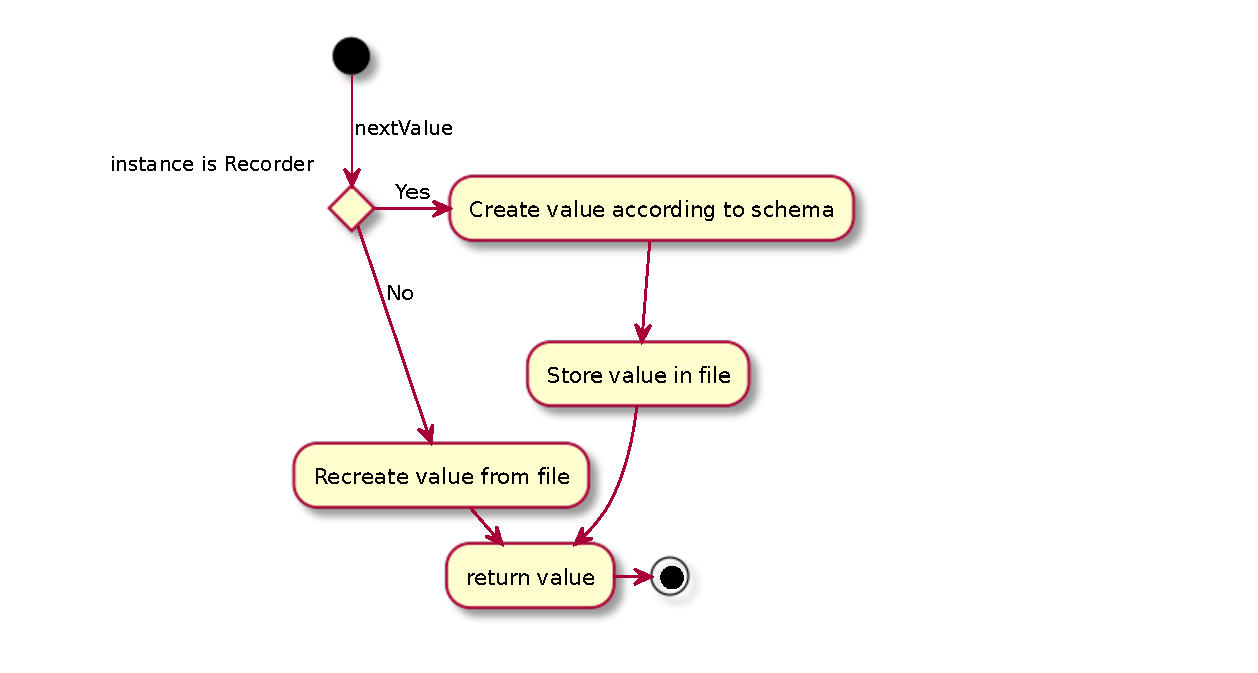
\includegraphics[width=.75\textwidth]{images/extensions/generalGeneratorWorkflow}
  \caption{Activity diagram showing how the generators will work.}
  \label{fig:generalGeneratorWorkflow}
\end{figure}

\section{Execution Tool}
\label{ch:design:se:executionTool}
YCSB has a script to run one workload on one database.
We have many workloads and multiple databases,
therefore it would save us a lot of time during evaluation,
if the workloads are executed on all databases sequentially.

That could be implemented as a script that takes the databases and their parameters together with the workload description files and executes one after another.
The results should be saved in a specified folder.

\section{Evaluation Tool}
\label{ch:design:se:evaluationTool}
To gather the results another script should iterate through the result folders of each database and workload and collect the results in a file for further evaluation.
     % Entwurf
\chapter{Implementation}
\label{ch:implementation}
In this chapter we will cover how we implemented the different classes to execute our workloads.
We will start with the graph and its components,
then move on to the different generators for the graph data,
the random graph components and the operation order.
Then we will show the workload class in section~\ref{ch:implementation:se:graphWorkload} and finally describe the database bindings in section~\ref{ch:implementation:se:graphDatabaseBindings}.

The code of our implementation is available on GitHub\footnote{\url{https://github.com/ChristianNavolskyi/YCSB}}.

In figure~\ref{fig:YCSBExtension} we see a diagram of the YCSB benchmark with our added implementations.
The classes we added are inside the red border on the right side.
In \texttt{Package db} we added the bindings for our four databases.

\begin{figure}
  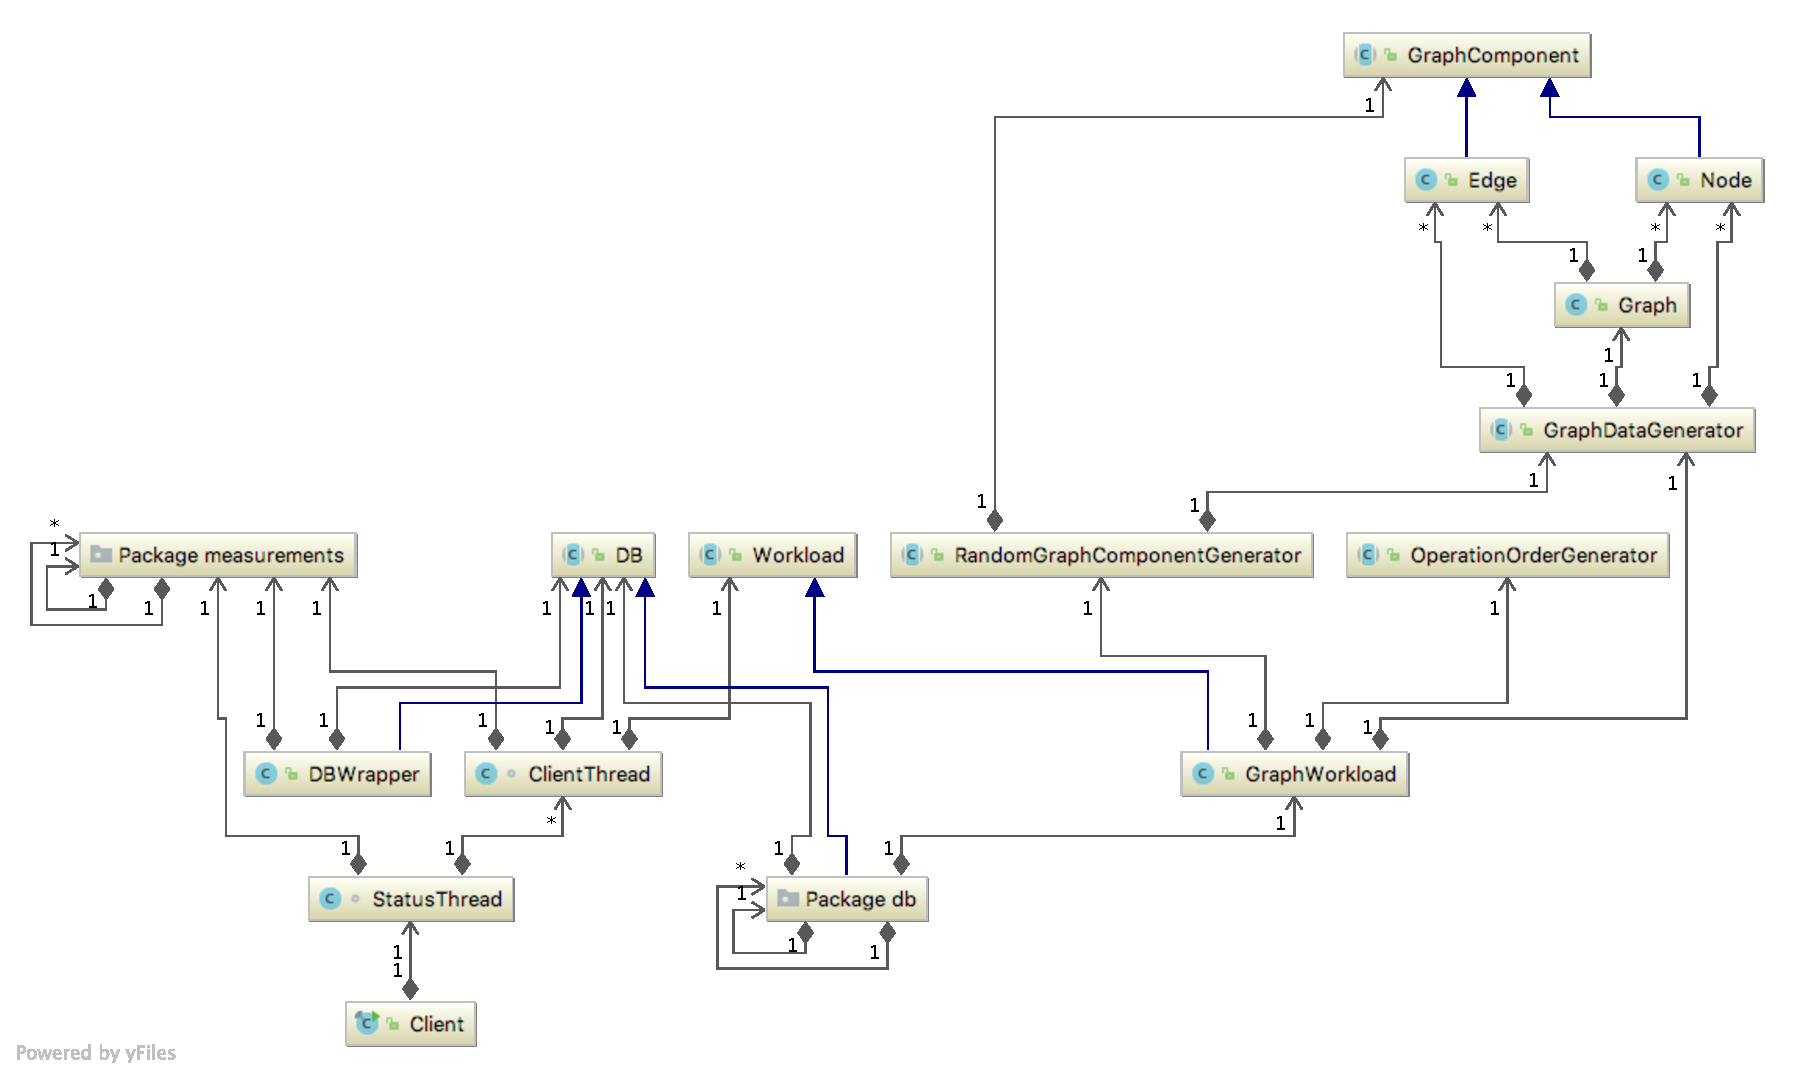
\includegraphics[angle=90,height=\textheight]{images/benchmarks/extendedYCSBWorkflow}
  \caption{Class diagram of YCSB with the most important classes we added to it placed inside the red border.}
  \label{fig:YCSBExtension}
\end{figure}

\section{Graph}
As mentioned in section~\ref{ch:background:se:graphs} a graph simply contains two lists,
one for nodes and one for edges.
This class is only a container for those two lists.

To extract some shared values of nodes and edges,
we added an abstract class \texttt{GraphComponent},
that holds the identifier and the label of the graph component.

\subsection{Node}
The \texttt{Node} class assigns the identifiers by counting the created nodes and incrementing the counter for every new node.
If the property value of a node isn't set,
a call to \texttt{Node::getHashMap} will randomly fill the property with the amount of characters specified by the \texttt{nodePropertySize} parameter.

\subsection{Edge}
As the \texttt{Node} class the \texttt{Edge} class also uses a counter field to assign the correct identifier to each edge.
Additionally,
the ids of the start and end \texttt{Node} are stored in fields.

\section{Generator}
\label{ch:implementation:se:generator}
The general workflow of a generator was mentioned at the end of section~\ref{ch:design:se:summary}.
Because all three generators share that behaviour we created an abstract class \texttt{StoringGenerator}\footnote{com.yahoo.ycsb.generator.StoringGenerator},
that extends the generic \texttt{Generator<V>}\footnote{com.yahoo.ycsb.generator.Generator} class and adds methods to check if the files are present for recreation or not.

Every generator offers a \texttt{create} method,
in which it will check for present files and set up the correct implementation (recorder or recreator) for the \texttt{GraphWorkload}\footnote{com.yahoo.ycsb.workloads.GraphWorkload}.
The generator classes are all abstract and use abstract methods to call the underlying implementation.
How this is useful will be described in the implementations of the different kinds of generators.

The abstract generator classes also contain the values needed for both implementation types (recorder and recreator),
to avoid code duplication.

\subsection{Graph Data}
The \texttt{nextValue} call encapsulates the call to get the subgraph from the underlying implementation and also stores the returned identifiers of the created nodes and edges for the \texttt{RandomGraphComponentGenerator}\footnote{com.yahoo.ycsb.generator.graph.randomcomponents.RandomGraphComponentGenerator}.

The \texttt{Gson}\footnote{com.google.gson.Gson} used in both implementations of this abstract class is initialised here with the \texttt{GraphAdapter}\footnote{com.yahoo.ycsb.generator.graph.GraphAdapter}.

Since there are two phases of the benchmark (see section~\ref{ch:analysis:se:ycsb}) the generator needs to know from what point it should move on with creation.
When the current phase is the transaction phase,
it will call the underlying implementation to create the amount of data that was created during the load phase,
to equalise the progress of the generator.
That is also important for the \texttt{RandomGraphComponentGenerator},
because the identifiers of the graph components created by the \texttt{GraphDataGenerator} are kept there for it to use them.

\subsection{Random Graph Component}
Calling \texttt{nextValue} on a \texttt{RandomGraphComponentGenerator} will invoke the implementing class to choose between a node and an edge.
Then a random graph component of that type is chosen.
A random node can also be picked directly,
as it's needed for the \texttt{GraphWorkload::update} method,
since it only will use nodes.

\subsection{Operation Order}
Here the generator only holds common fields shared by the recorder and the recreator.

\section{Recorder}
\label{ch:implementation:se:recorder}
For every generator we have a creator that creates the initial values for the workload and stores them in a corresponding file for the recreator presented in section~\ref{ch:implementation:se:recreator}.

How the creation of the values is implemented in each generator is described in the following subsections~\ref{ch:implementation:se:graphDataRecorder}~to~\ref{ch:implementation:se:operationOrderRecorder}.

\subsection{Graph Data}
\label{ch:implementation:se:graphDataRecorder}
As shown in figure~\ref{fig:generalGeneratorWorkflow} when \texttt{GraphDataGenerator::nextValue}\footnote{com.yahoo.ycsb.generator.graph.GraphDataGenerator} is called to create the next subgraph,
the \texttt{GraphDataRecorder} is called and creates the subgraph according to the diagram shown in figure~\ref{fig:graphDataRecorder}.
Each subgraph is then serialised and the string coming from serialisation is written into a file line by line.

Table~\ref{tab:recorderVariables} shows how the parameters x, y and z of the data structure from figure~\ref{fig:finalDesignOfSchema} are implemented in that schema.
They all affect when the specific if block is executed at the end of figure~\ref{fig:graphDataRecorder} to reset the corresponding values for the if blocks above.\\
The creation of a subgraph can be seen in a loop,
in every iteration another if-condition is fulfilled to return the next value.

\begin{figure}[h!]
  \centering
  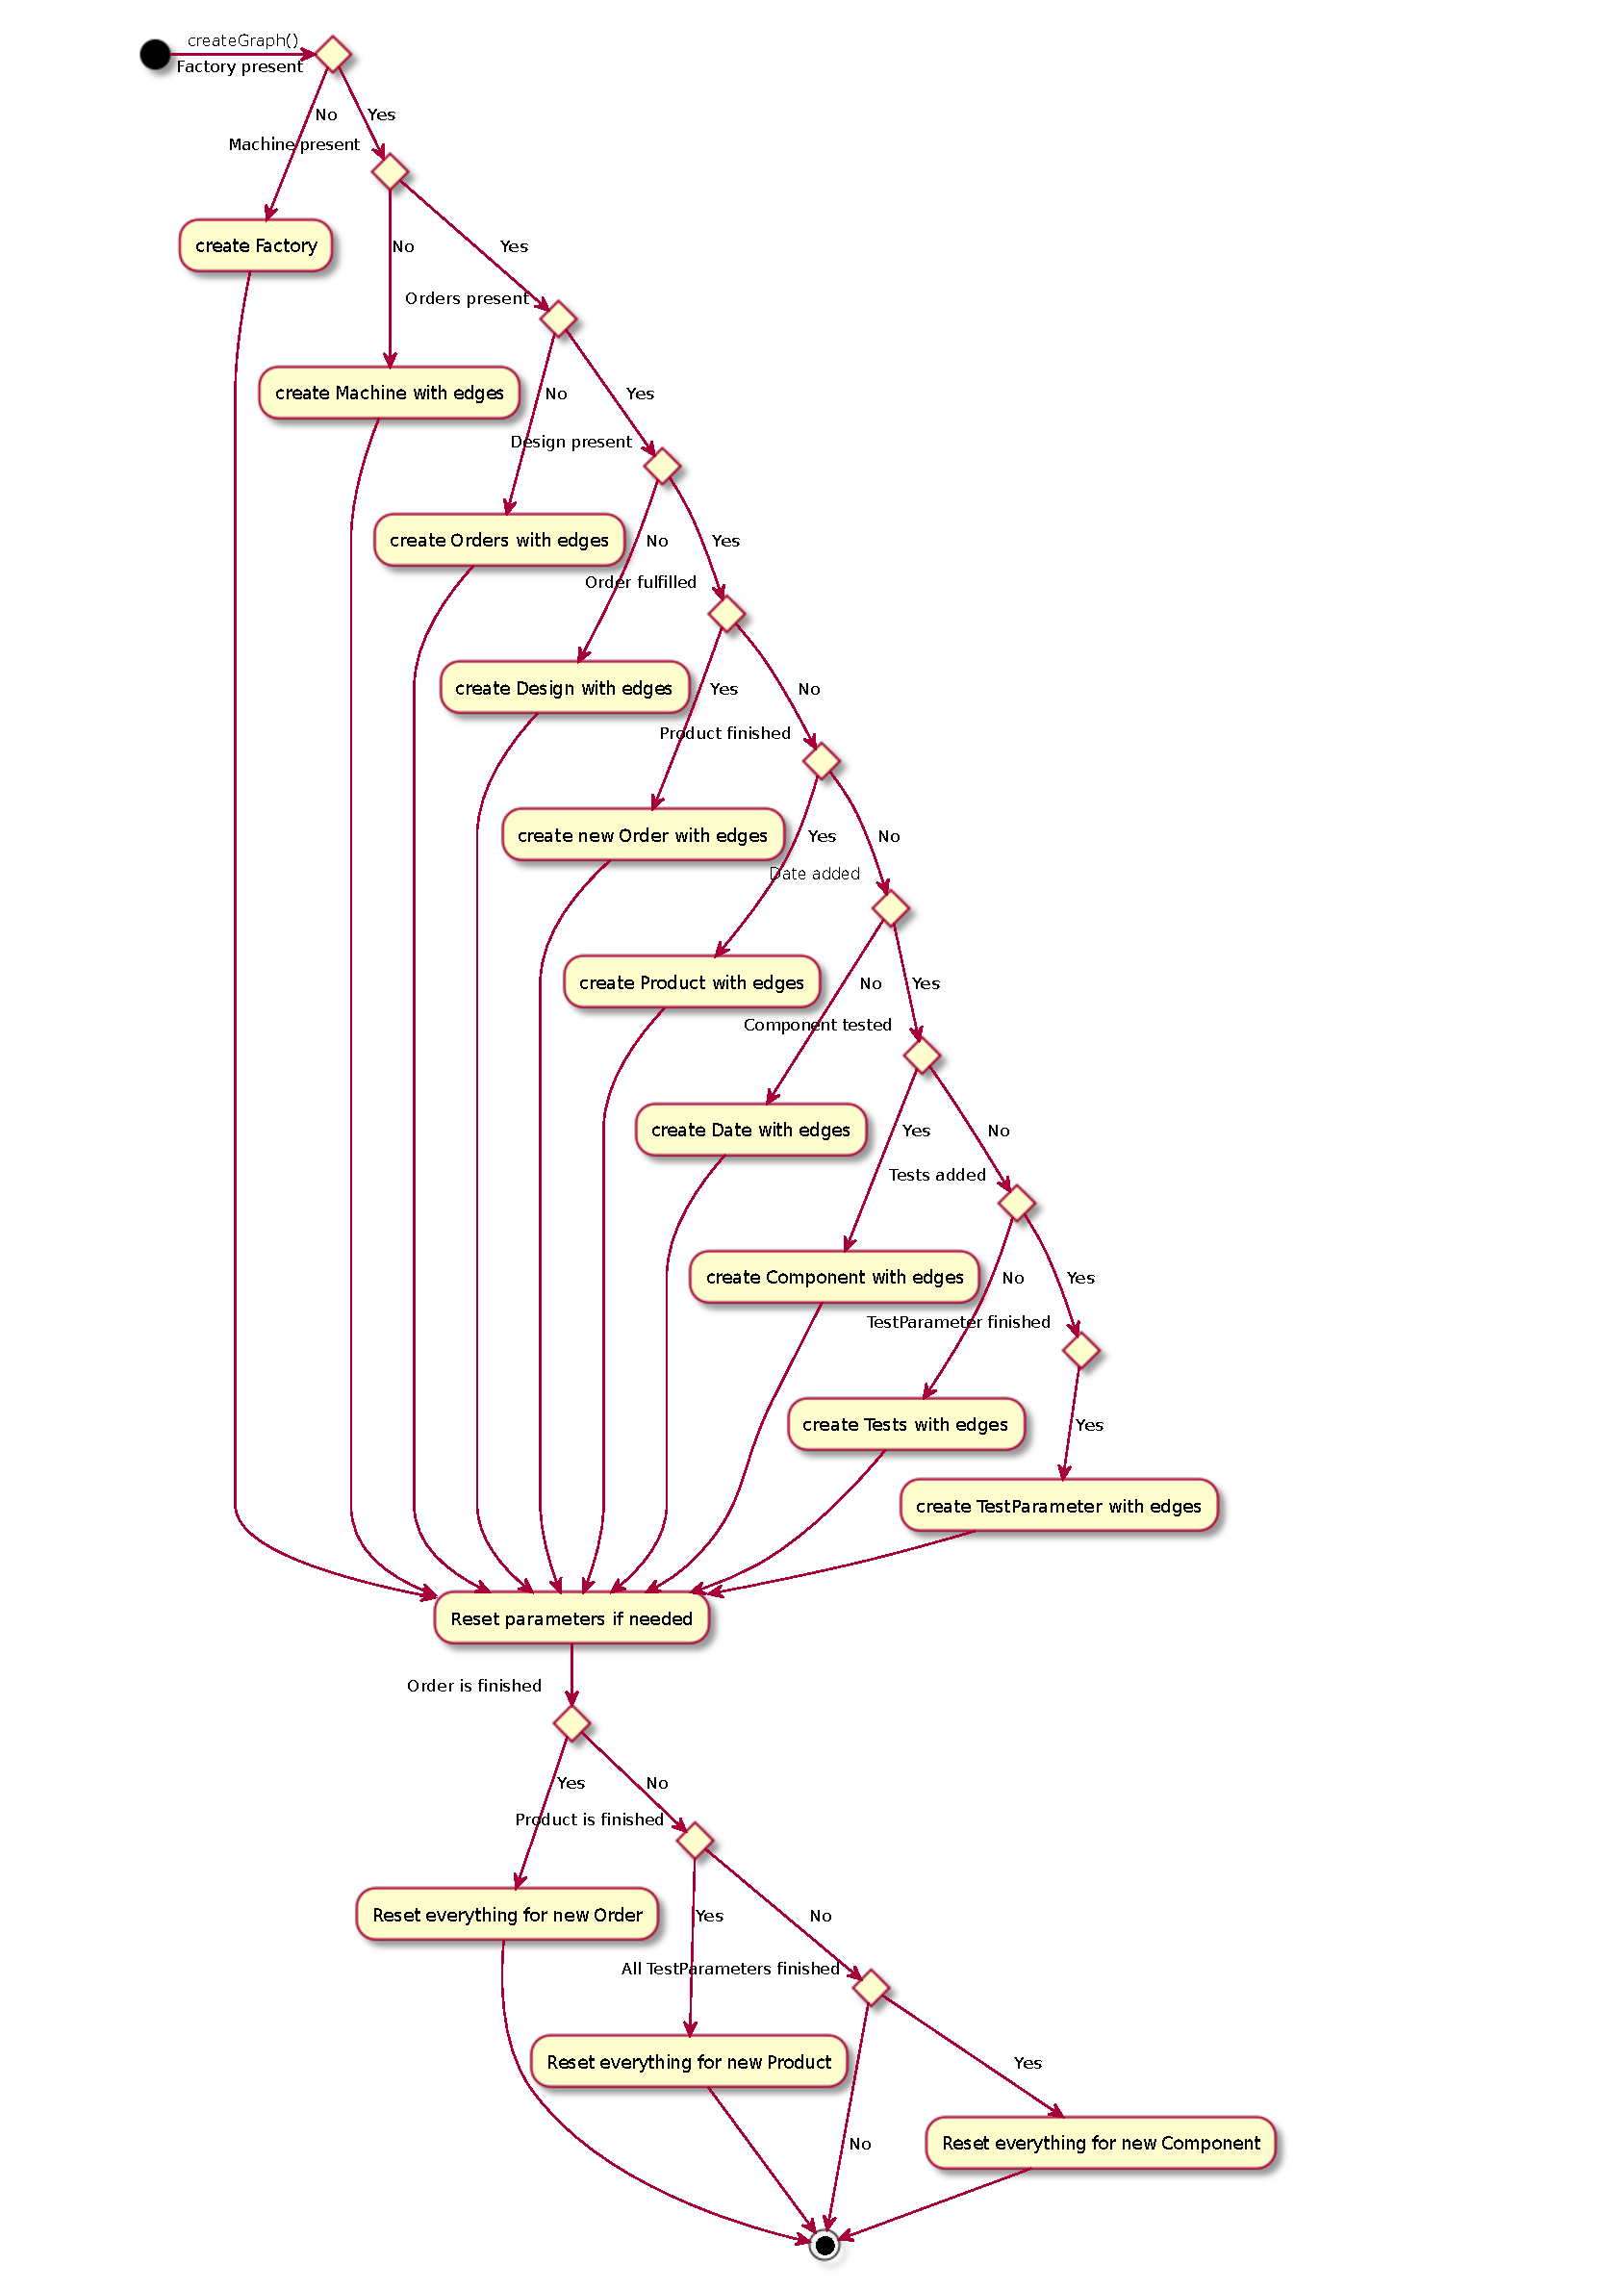
\includegraphics[width=\textwidth]{images/extensions/GraphDataRecorder}
  \caption{Activity diagram of the creation process for the dataset.}
  \label{fig:graphDataRecorder}
\end{figure}

\begin{table}[h!]
  \begin{tabularx}{\textwidth}{ | l | X | }
    \hline
    Variable & Usage \\ \hline \hline
    x & Determines after how many products the order is fulfilled \\ \hline
    y & Determines after how many components a product is finished \\ \hline
    z & Determines after how many tests all test parameters are finished \\ \hline
  \end{tabularx}
  \caption{Implementation of the structure variables in the creation of the dataset.}
  \label{tab:recorderVariables}
\end{table}

The serialisation process is done in the \texttt{GraphAdapter} that implements both a \texttt{JsonSerializer}\footnote{com.google.gson.JsonSerializer} and a \texttt{JsonDeserialzer}\footnote{com.google.gson.JsonDeserialzer} with a \texttt{Graph} as the generic argument.
Since a graph object contains two lists,
these lists are serialised into \texttt{JsonElement}s\footnote{com.google.gson.JsonElement},
which will be retrieved as a string by calling \texttt{Gson::toJsonTree}.
The following listing~\ref{lst:serialiseCode} shows the Java code used to implement the serialisation of a graph.

\begin{lstlisting}[language=Java,label={lst:serialiseCode},caption={Serialisation of a \texttt{Graph} object.},captionpos=b]
@Override
public JsonElement serialize(Graph graph, Type typeOfSrc, JsonSerializationContext context) {
 JsonObject result = new JsonObject();

 JsonElement nodeJsonElement = gson.toJsonTree(graph.getNodes(), nodeListType);
 JsonElement edgeJsonElement = gson.toJsonTree(graph.getEdges(), edgeListType);

 result.add(nodes, nodeJsonElement);
 result.add(edges, edgeJsonElement);

 return result;
}
\end{lstlisting}

\subsection{Random Graph Component}
To choose between a node and an edge a random number between zero and one will be picked ($ r \in \mathbb{N}_0 \wedge r \in [ 0, 1 ] $) and stored in a file.
To select a random graph component the \texttt{GraphDataGenerator} will be asked what the last id was and then a random value between zero and that number will be generated.
That value will also be stored in a file corresponding to the type of the graph component.

\subsection{Operation Order}
\label{ch:implementation:se:operationOrderRecorder}
The \texttt{OperationOrderRecorder}\footnote{com.yahoo.ycsb.generator.operationorder.OperationOrderGenerator} receives a \texttt{DiscreteGenerator}\footnote{com.yahoo.ycsb.generator.DiscreteGenerator},
which supplies the string values for the operations that will be saved in a file and then returned to the caller.

\section{Recreator}
\label{ch:implementation:se:recreator}
To retrieve the values stored by the recorder classes described in section~\ref{ch:implementation:se:recorder} the upcoming recreators are needed.

\subsection{Graph Data}
If the files for the dataset are present the \texttt{GraphDataRecreator} will be called to return the next subgraph.
It does that by deserialising the next line with the \texttt{Gson::fromJson} method which uses the \texttt{GraphAdapter} described in subsection~\ref{ch:implementation:se:graphDataRecorder} together with a \texttt{Type}\footnote{java.lang.reflect.Type}.
The code of the \texttt{GraphAdapter} to deserialise a \texttt{Graph} is shown in listing~\ref{lst:deserialiseGraph}.

\begin{lstlisting}[language=Java,label={lst:deserialiseGraph},caption={Deserialisation of a \texttt{Graph} object.},captionpos=b]
@Override
public Graph deserialize(JsonElement jsonElement, Type type, JsonDeserializationContext context) throws
    JsonParseException {
  Graph graph = new Graph();
  JsonObject jsonObject = jsonElement.getAsJsonObject();

  JsonElement jsonNodes = jsonObject.get(nodes);
  JsonElement jsonEdges = jsonObject.get(edges);

  List<Node> nodeList = gson.fromJson(jsonNodes, nodeListType);
  List<Edge> edgeList = gson.fromJson(jsonEdges, edgeListType);

  nodeList.forEach(graph::addNode);
  edgeList.forEach(graph::addEdge);

  return graph;
}
\end{lstlisting}

This class uses a \texttt{BufferedReader}\footnote{java.io.BufferedReader} to read the file line by line,
to avoid extensive memory usage with larger datasets.

\subsection{Random Graph Component}
\label{ch:implementation:se:randomGraphComponentRecreator}
At the beginning the files will be read and their values will be stored in three different \texttt{Iterator<String>}s\footnote{java.util.Iterator<E>},
one for the type and the other two for the identifiers of the different kinds of graph components.

When a value is required the corresponding \texttt{Iterator<String>} returns the next value in the list and increments its pointer.

\subsection{Operation Order}
As the \texttt{RandomGraphComponentRecreator} from subsection~\ref{ch:implementation:se:randomGraphComponentRecreator},
this recreator reads the file directly during initialisation and stores the values in an \texttt{Iterator<String>}.

Every time \texttt{OperationOrderRecreator::nextValue} is called the next line from the \texttt{Iterator<String>} is returned.

\section{Graph Workload}
\label{ch:implementation:se:graphWorkload}
During initialisation the \texttt{GraphWorkload} creates the three generators mentioned in section~\ref{ch:implementation:se:generator},
by using the \texttt{create} method.
That way it will receive the correct type (recorder or recreator) for each generator.
This process is shown in figure~\ref{fig:graphWorkloadInit}

\begin{figure}[h!]
  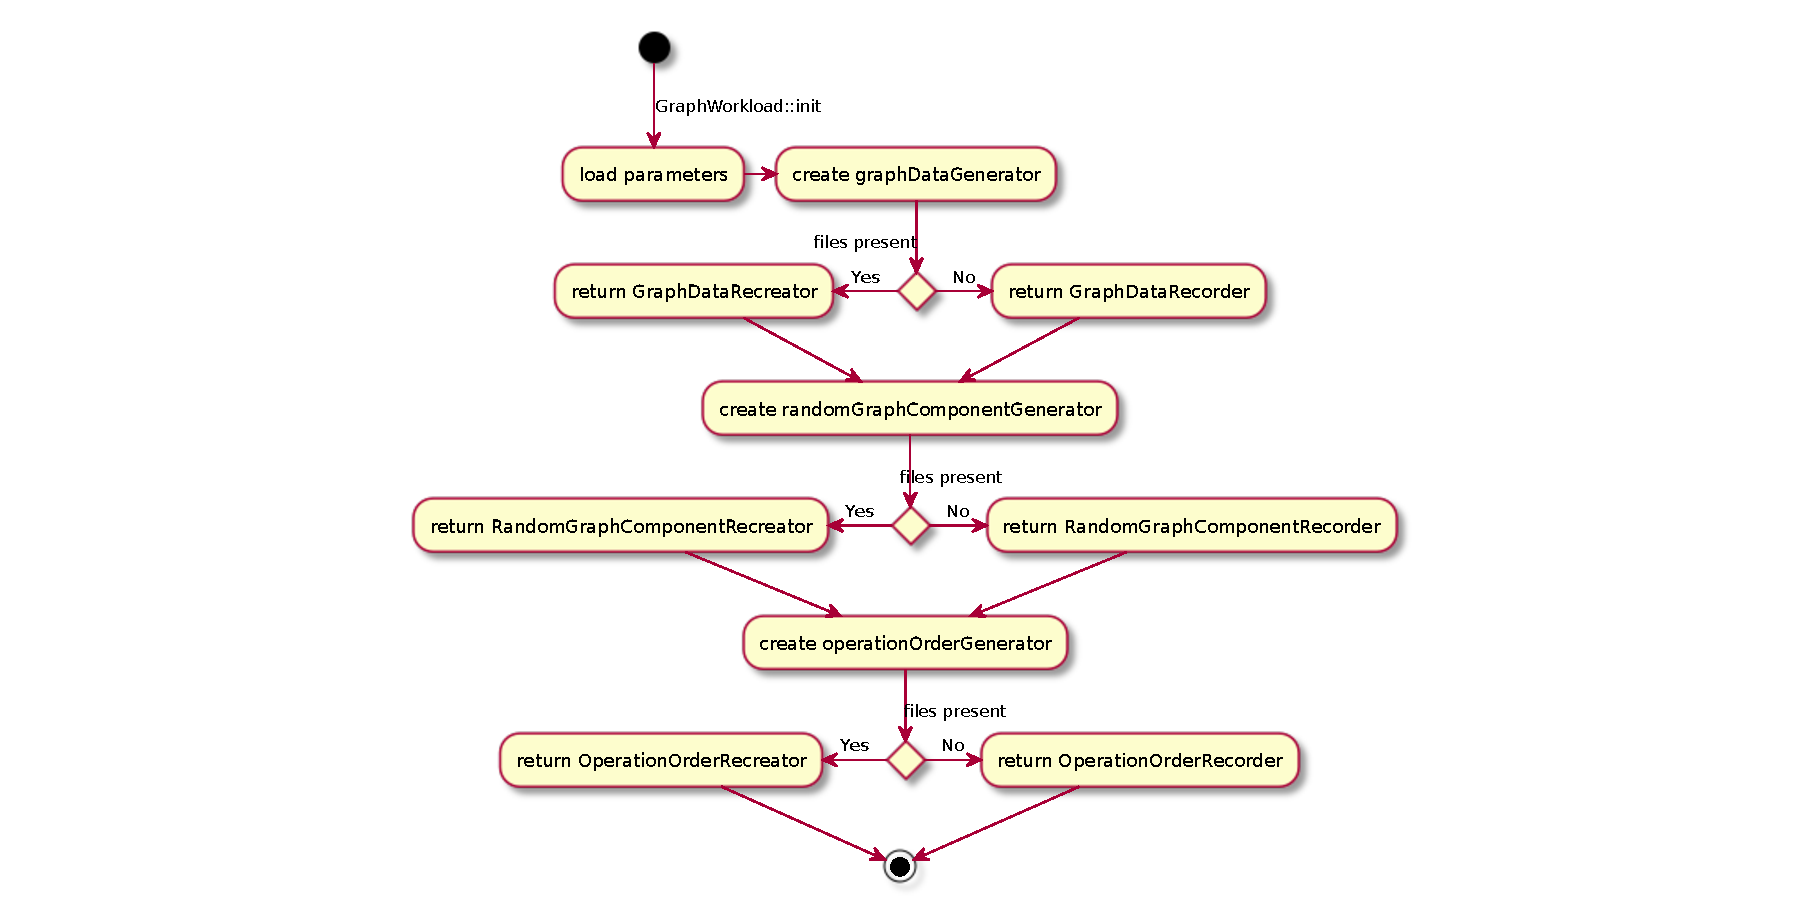
\includegraphics[width=\textwidth]{images/extensions/GraphWorkload}
  \caption{Initialisation of the generators used in the \texttt{GraphWorkload}.}
  \label{fig:graphWorkloadInit}
\end{figure}

It also parses the parameters to get the values for \texttt{noEdges},
the \texttt{property size} of a node,
how many fields should be scanned (\texttt{recordcount}) and the \texttt{folder}.
The \texttt{noEdges} parameter is needed to execute the operations on the correct available graph components.
The \texttt{property size} is stored to be retrievable by the \texttt{Node} to know how many random characters it should generate.
The \texttt{recordcount} option is needed for the \texttt{scan} operation.
Lastly the \texttt{folder} is used to create the folder for the dataset if it isn't present and also pass it to the individual generators.

In the load phase the \texttt{Client}\footnote{com.yahoo.ycsb.Client} calls \texttt{GraphWorkload::doInsert}.
The \texttt{GraphWorkload} then retrieves a subgraph from the \texttt{GraphDataGenerator} by calling \texttt{GraphDataGenerator::nextValue},
separates it into its graph components and calls the \texttt{DB::insert} method with each individual component to add them to the database one by one.

If the \texttt{Client} calls \texttt{GraphWorkload::doTransaction} the \texttt{GraphWorkload} will first get the operation to execute on the database by the \texttt{OperationOrderGenerator}.
After that it has an implementation for every available database operation.
The general workflow for the \texttt{GraphWorkload::doTransaction} method is shown in figure~\ref{fig:graphWorkloadExecution}.

\begin{figure}[h!]
  \includegraphics[width=\textwidth]{images/extensions/graphWorkloadExecution}
  \caption{Overview of the execution of the different database operations separated into insert and other operations.}
  \label{fig:graphWorkloadExecution}
\end{figure}

\textbf{doTransactionInsert} \newline
Works as in the \texttt{doInsert} method,
by taking a subgraph from the \texttt{GraphDataGenerator} and inserting its components one by one into the database.

\textbf{doTransactionRead} \newline
Depending on the \texttt{noEdges} option the \texttt{RandomGraphComponentGenerator} will be asked for a graph component,
if the option is \texttt{false} and a node if the option is \texttt{true}.
With the identifier of the graph component,
its type and its available fields the database is queried to look up those fields of the specified component.

\textbf{doTransactionScan} \newline
As in the \texttt{doTransactionRead} method a graph component is chosen from the \texttt{RandomGraphComponentGenerator} depending on the set \texttt{noEdges} option.
Then the necessary arguments from the graph component will be passed to the \texttt{DB::scan} method,
alongside the specified \texttt{recordcount}.

\textbf{doTransactionUpdate} \newline
The \texttt{update} method isn't used by our workloads,
but to make the \texttt{GraphWorkload} accessible to other workloads we implemented it as follows.
A random graph component is picked and the \texttt{DB::update} method of the database is called.
If the graph component is a node its property value will be randomly assigned.

We didn't implement the \texttt{delete} method of the database,
as we won't use it in our workloads and the \texttt{CoreWorkload} that we used as reference also didn't use it.

\subsection{Parameters}
This subsection covers the naming of the parameters in the code.

\begin{table}[h!]
  \begin{minipage}{\textwidth}
    \begin{tabularx}{\textwidth}{ | X | X | }
      \hline
      Our name & Name in the code \\ \hline \hline
      folder & datasetdirectory \\ \hline
      productsPerOrder & productsperorder \\ \hline
      componentsPerProduct & componentsperproduct \\ \hline
      testParameterCount & testparametercount \\ \hline
      recordcount & maxscanlength \\ \hline
      noEdges & onlynodes \\ \hline
      nodePropertySize & fieldlength \\ \hline
    \end{tabularx}
  \end{minipage}
  \caption{This table shows the name the parameters as they can be found in the YCSB project.}
  \label{tab:parameterMapping}
\end{table}

The \texttt{dbFolder} option is different for each database and will be mentioned in the corresponding binding subsection.
The same goes for the \texttt{useIndex} option.

\section{Graph Database Bindings}
\label{ch:implementation:se:graphDatabaseBindings}
In this section we will describe the different binding implementations, their specialities and how they implemented the different operations mentioned in section~\ref{ch:design:se:bindings}.
Table~\ref{tab:bindingParameterMapping} shows the available options for the different databases.

\begin{table}[h!]
  \begin{minipage}{\textwidth}
    \begin{tabularx}{\textwidth}{ | X | X | X | }
      \hline
      Database & Folder option & Index option \\ \hline \hline
      Apache Jena & outputdirectory & - \\ \hline
      Neo4j & neo4j.path & neo4j.index \\ \hline
      OrientDB & orientdb.url & orientdb.index \\ \hline
      Sparksee & sparksee.path & sparksee.index \\ \hline
    \end{tabularx}
  \end{minipage}
  \caption{Parameter names of the different databases for the database folder and the index option.}
  \label{tab:bindingParameterMapping}
\end{table}

At the beginning of each subsection we will show how we initialised the database and how the instance to work with the database is retrieved.

\subsection{Apache Jena}
In the following listing~\ref{lst:jenaInit} the initialisation and the beginning of a transaction with the retrieval of a model to work on the data is shown.

\begin{lstlisting}[language=Java,label={lst:jenaInit},caption={Implementation of the initialisation and model retrieval in Jena.},captionpos=b]
String outputDirectory = getDirectoryFromProperties();
Dataset dataset = TDBFactory.createDataset(outputDirectory); // Create dataset, represents the database.

dataset.begin(ReadWrite.WRITE); // Starts a write transaction, ReadWrite.READ is used for read operations.

try {
  Model model = dataset.getDefaultModel(); // Needed to access the database.

  performOpertaionOnModel();

  dataset.commit();
} finally {
  dataset.end(); // Finish transaction.
}
\end{lstlisting}

To modify the database with Jena we need to start a transaction and specify whether it is a read or a write transaction.
After that we retrieve the model of the database to work on the data.
After we are done with our operation we need to commit or abort the transaction,
similar to a relational database.

\textbf{creating a node} \newline
A node is created by calling \texttt{Model::createResource}\footnote{org.apache.jena.rdf.model.Model} with an \texttt{AnonId}\footnote{org.apache.jena.rdf.model.AnonId} that receives the \texttt{key} as an argument.

\textbf{creating an edge} \newline
To create an edge we use the \texttt{Model::createProperty} method with the \texttt{key} as the argument.
To connect the edge with their start and end node,
we have to add this triple to the model by calling \texttt{Model::add} with the start node,
the edge and the end node.

\textbf{adding properties to a node} \newline
Properties are mapped as statements in Jena and to create those we use the
\texttt{Model::\allowbreak createStatement} method that takes the node, the key for the property and the property value as arguments.
After all statements are created we add them to the model with \texttt{Model::add} and the list of statements as the argument.

\textbf{adding properties to an edge} \newline
To add properties to an edge,
we use the \texttt{Property::addProperty} method on it with the key of the property and its value as the arguments.

\textbf{getting a node by its identifier} \newline
Retrieving a node is done by creating a resource with the same identifier.
Jena will look up the database whether one already exists,
and the returned node will be equal to an existing one.

\textbf{getting an edge by its identifier} \newline
Similar to retrieving a node from the database we create a property with the \texttt{key},
that returns an existing edge if one exists for that \texttt{key}.

\textbf{getting the values of a node/an edge} \newline
To get the values associated with a node,
we create a \texttt{SimpleSelector}\footnote{org.apache.jena.rdf.model.SimpleSelector},
which can be used as a query on the database.
We supply it the node and the key of the value and leave the object of the query empty,
so it looks up the matching values for the object.

\textbf{getting the outgoing edges of a node} \newline
To get these edges we list the properties of the node.

\textbf{getting the start node of an edge} \newline
To do this,
we take the start property of the edge and look up that node on the dataset.

\textbf{removing a node} \newline
Removing a node is done by calling \texttt{Model::removeAll} twice,
once with the node as the subject and once with the node as the object of the statement.
That will remove all statements associated with that node,
which effectively removes the node from the database.

\textbf{removing an edge} \newline
Here we also call \texttt{Model::removeAll} but the with edge as the predicate of the statement.

\subsection{Neo4j}
If an \texttt{Index}\footnote{org.neo4j.graphdb.index.Index<T extends PropertyContainer>} should be used we create two of them,
one for \texttt{Node}s\footnote{org.neo4j.graphdb.Node} and one for \texttt{Relationship}s\footnote{org.neo4j.graphdb.Relationship} (edges).
Neo4j also uses transaction,
but we don't need to specify their kind.
At the end of a transaction we call \texttt{Transaction::success}\footnote{org.neo4j.graphdb.Transaction} to finish the transaction.

An example of our implementation is shown in the following listing~\ref{lst:neo4jInit}.
The start and end of a transaction for an operation are implemented as in the if-block of the listing.

\begin{lstlisting}[language=Java,label={lst:neo4jInit},caption={Implementation of the initialisation and beginning of a transaction.},captionpos=b]
String path = getPathFromProperties();
boolean useIndex = shouldUseIndex();

GraphDatabaseService graphDbInstance = new GraphDatabaseFactory().newEmbeddedDatabase(new File(path)); // Creates to object to access the database.

if (useIndex) {
  try (Transaction transaction = graphDbInstance.beginTx()) { // Start a transaction.
    IndexManager index = graphDbInstance.index();
    nodeIndex = index.forNodes("nodes");
    relationshipIndex = index.forRelationships("relationships");
    transaction.success(); // End a transaction.
  }
}
\end{lstlisting}

\textbf{creating a node} \newline
We create a node with the \texttt{GraphDatabaseService::createNode}\footnote{org.neo4j.graphdb.GraphDatabaseService} method,
where we specify the \texttt{key} as the \texttt{Label}\footnote{org.neo4j.graphdb.Label} of the node.
If an \texttt{Index} is used,
we add the node to the index after creation.
After that we add the identifier of the node as a property to be able to look the node up by its identifier.

\textbf{creating an edge} \newline
For this we have to first create a \texttt{RelationshipType}\footnote{org.neo4j.graphdb.RelationshipType} with the \texttt{key} as the name of the relationship.
Then we create a relationship from the start node to the end node by calling \texttt{Node::createRelationshipTo}.
Finally,
we add the edge to the relationship \texttt{Index}.

\textbf{adding properties to a node/an edge} \newline
Both \texttt{Node}s and edges are \texttt{PropertyContainer}s\footnote{org.neo4j.graphdb.PropertyContainer},
which support the setting of properties,
by calling \texttt{PropertyContainer::setProperty} with the key of the property and its value.

\textbf{getting a node by its identifier} \newline
When an \texttt{Index} is used a node can be looked up on it with \texttt{Index::get},
the key for the identifier and the identifier value.
Without an \texttt{Index} we call \texttt{GraphDatabaseService::findNode} with the \texttt{Label},
the key for the identifier and the identifier as arguments.

\textbf{getting an edge by its identifier} \newline
With an \texttt{Index} a \texttt{Relationship} can be found similar to a node.
Without an index we have to iterate over all \texttt{Relationship}s in the graph and check their types to match the \texttt{key}.

\textbf{getting the values of a node/an edge} \newline
The \texttt{PropertyContainer::getAllProperties} method supplies all values set to the node or edge.
We can simply parse the \texttt{Map<String, Object>}\footnote{java.util.Map<K, V>} returned by it to the needed \texttt{Map<String, ByteIterator>}.

\textbf{getting the outgoing edges of a node} \newline
\texttt{Node}s offer a method to get their \texttt{Relationship}s in a specified \texttt{Direction}\footnote{org.neo4j.graphdb.Direction} with \texttt{Node::getRelationships}.

\textbf{getting the start node of an edge} \newline
\texttt{Relationship}s also offer a method to directly get their start node with \texttt{Relationship::getStartNode}.

\textbf{removing a node/an edge} \newline
To remove a \texttt{Node} or a \texttt{Relationship},
we look it up,
remove it from the corresponding \texttt{Index} and then call \texttt{Node::delete} or \texttt{Relationship::delete} respectively,
to remove it from the database.

\subsection{OrientDB}
To create an index in OrientDB we call \texttt{OrientGraph::createKeyIndex}\footnote{com.tinkerpop.blueprints.impls.orient.OrientGraph} with the key of the identifier and the graph component classes,
once with \texttt{Vertex}\footnote{com.tinkerpop.blueprints.Vertex} and once with \texttt{Edge}\footnote{com.tinkerpop.blueprints.Edge}.
As Neo4j OrientDB uses transactions to execute operations on the database,
which have to be closed after finishing the operation by calling \texttt{OrientGraph::shutdown}.

An example of our implementation covering the initialisation and retrieval of an \texttt{OrientGraph} for a transaction is shown in listing~\ref{lst:orientdbInit}.

\begin{lstlisting}[language=Java,label={lst:orientdbInit},caption={Implementation of the initialisation and the retrieval of an \texttt{OrientGraph} for a transaction.},captionpos=b]
String url = getURLFromProperties();

OrientGraphFactory factory = new OrientGraphFactory(url, userName, password); // Create object to access database.

if (useIndex) {
  OrientGraph graph = factory.getTx(); // Start a transaction.
  if (graph.getIndexedKeys(Vertex.class).size() == 0) {
    graph.createKeyIndex(nodeIdIdentifier, Vertex.class);
  }

  if (graph.getIndexedKeys(com.tinkerpop.blueprints.Edge.class).size() == 0) {
    graph.createKeyIndex(edgeIdIdentifier, com.tinkerpop.blueprints.Edge.class);
  }
}

try {
  performOperationOnGraph();
} finally {
  graph.shutdown(); // End a transaction.
}
\end{lstlisting}

\textbf{creating a node} \newline
To add a node,
we simply call \texttt{OrientGraph::addVertex} with the \texttt{key} and the \texttt{value} map we want to put in.
Before we add the value map,
we have to transform the \texttt{ByteIterator}\footnote{com.yahoo.ycsb.ByteIterator} values to \texttt{String}s with the \texttt{Object::toString} method.

\textbf{creating an edge} \newline
An edge is created by calling \texttt{OrientGraph::addEdge} with the \texttt{key},
the start node,
the end node and a label,
which we will simply set to "Edge",
because the label of our \texttt{values} map will be set as a property.

\textbf{adding properties to a node} \newline
As mentioned in "creating a node",
the values for the properties are directly passed during creation.

\textbf{adding properties to an edge} \newline
We can add the \texttt{values} to an edge by calling \texttt{OrientElement::setProperties}\footnote{com.tinkerpop.blueprints.impls.orient.OrientElement} with the map of string values.

\textbf{getting a node by its identifier} \newline
A node is looked up by \texttt{OrientGraph::getVertices} with the identifier key and the identifier value.

\textbf{getting an edge by its identifier} \newline
\texttt{Edge}s can be retrieved similarly,
by calling \texttt{OrientGraph::getEdges} with the according parameters.

\textbf{getting the values of a node/an edge} \newline
The properties of an \texttt{OrientElement} can be obtained by calling
\texttt{OrientElement::\allowbreak getProperties}.
The values of the returned map are then cast to \texttt{ByteIterator}s.

\textbf{getting the outgoing edges of a node} \newline
The edges of a node can be gathered by calling \texttt{OrientVertex::getEdges} with the specified direction.

\textbf{getting the start node of an edge} \newline
The procedure is analogous to that of getting the outgoing edge of a node.
We call \texttt{OrientEdge::getVertex} with the specified direction.

\textbf{removing a node} \newline
The \texttt{OrientGraph::removeVertex} method can be used to delete a vertex from the database.

\textbf{removing an edge} \newline
As to remove a node,
the \texttt{OrientGraph} provides a method to remove an edge internally,
that means the connected nodes aren't removed.

\subsection{Sparksee}
The index can be activated on certain attributes by calling \texttt{Graph::indexAttribute}\footnote{com.sparsity.sparksee.gdb.Graph} with the attribute and \texttt{AttributeKind.Indexed}\footnote{com.sparsity.sparksee.gdb.AttributeKind} as arguments.
Sparksee uses \texttt{Session}s\footnote{com.sparsity.sparksee.gdb.Session} as transaction,
these have to be closed at the end of a transaction.

In the following listing~\ref{lst:sparkseeInit} we show how we implemented the initialisation, the activation of an index and the retrieval of a graph instance to work on the database.
After the graph is retrieved any operations on the database can be executed,
in our example we initialised the index.

\begin{lstlisting}[language=Java,label={lst:sparkseeInit},caption={Implementation of the initialisation and starting of a session.},captionpos=b]
String path = getPathFromProperties();
boolean useIndex = shouldUseIndex();

Sparksee sparksee = new Sparksee(new SparkseeConfig()); // Create object for database access.

if (new File(path).exists()) {
  database = sparksee.open(path, false);
} else {
  database = sparksee.create(path, "SparkseeDB");
}

try (Session session = database.newSession()) { // Start a transaction. The try-with-resource block closes the session automatically at the end.
  Graph graph = session.getGraph(); // Obtain Graph to work on the database.

  nodeIdAttribute = getAttribute(graph, getNodeType(graph), "sparksee.nodeId");
  edgeIdAttribute = getAttribute(graph, getEdgeType(graph), "sparksee.edgeId");

  if (useIndex) {
    try {
      graph.indexAttribute(nodeIdAttribute, AttributeKind.Indexed);
      graph.indexAttribute(edgeIdAttribute, AttributeKind.Indexed);
    } catch (RuntimeException e) {
      // The presence of an index cannot be queried, so we will catch and ignore the exception that is thrown when an index already exists.
      e.printStackTrace();
    }
  }
}
\end{lstlisting}

\textbf{creating a node} \newline
To create a node,
we first create a type for the node,
which is the same for all nodes.
Then we call \texttt{Graph::newNode} and set a identifier attribute to store the \texttt{key} in the node.

\textbf{creating an edge} \newline
Here we have to look up the two corresponding nodes and then create an edge type,
that is the same for all edges.
We then create an edge by calling \texttt{Graph::newEdge} with the type,
the start and the end node.
Lastly the identifier for the edge is set as an attribute.

\textbf{adding properties to a node/an edge} \newline
To add attributes,
we have to create an attribute in the database with the name of the property.
Then we call \texttt{Graph::setAttribute} with that attribute and its value.

\textbf{getting a node/an edge by its identifier} \newline
Retrieving a graph component works by creating a \texttt{Value}\footnote{com.sparsity.sparksee.gdb.Value} with the key of the component,
which is then passed to the \texttt{Graph::findObject} method with the attribute specifying a node or an edge identifier.

\textbf{getting the values of a node/an edge} \newline
The attributes of a graph component are obtained by calling \texttt{Graph::getAttributes},
which hands us an \texttt{AttributeList}\footnote{com.sparsity.sparksee.gdb.AttributeList} that is then looked up for the attributes we want.

\textbf{getting the outgoing edges of a node} \newline
To get the edges connected to a node,
we call \texttt{Graph::neighbors} with the node, the type of edge and the direction.

\textbf{getting the start node of an edge} \newline
The \texttt{EdgeData::getHead} method serves us the start node.

\textbf{removing a node/an edge} \newline
To remove a graph component from the database we look the component up and then call \texttt{Graph::drop} on it,
to delete it from the database.
    % Implementierung
\chapter{Evaluation}
\label{ch:evaluation}
This chapter will cover the execution and evaluation of our benchmark with the workloads specified in section~\ref{ch:design:se:workloads}.
We will present the results of each workload and have a discussion on them directly after that.

A conclusion will be drawn in section~\ref{ch:futureWork:se:conclusion} in the next chapter.

\section{Objective}
The main goal is to see,
if the databases are capable of handling the production workloads.
To test that feature we will also make some other performance benchmarks to be able to evaluate the write speeds of the databases.

We want to measure the average time needed for a single insert operation,
that way we can compare the databases without take into account the overhead of the benchmark itself,
which will be reflected in the overall run time.

For the workloads including read operations we will also look at the overall run time to get a better view on the impact these operations have on the performance.

In section~\ref{ch:evaluation:se:overview} we will show which workloads we will compare with each other and what we want to evaluate through that comparison.

\section{Setup}
In this section we will describe the software and hardware we used to execute the benchmark.

\subsection{Hardware}
The computer used for the benchmark had the specifications shown in table~\ref{tab:hardware}.

\begin{table}[!h]
  \begin{minipage}{\textwidth}
    \begin{tabularx}{\textwidth}{ | l | X | }
      \hline
      Component & Description \\ \hline \hline
      CPU & Intel i7-3770K @ 3.5GHz \\ \hline
      RAM & 16GB DDR3 @ 1.600MHz \\ \hline
      Storage & Seagate ST2000DL003 2 TB 5900rpm, only a 400GB partition was used \\ \hline
      GPU & NVIDIA GeForce GTX 670 \\ \hline
    \end{tabularx}
  \end{minipage}
  \caption{The hardware specifications of the computer for the benchmark.}
  \label{tab:hardware}
\end{table}

\subsection{Software}
The versions of the software components we used are shown in the following table.

\begin{table}[!h]
  \begin{minipage}{\textwidth}
    \begin{tabularx}{\textwidth}{ | X | X | }
      \hline
      Software & Version \\ \hline \hline
      Ubuntu & 17.10 \\ \hline
      Java & 1.8.0\_171 \\ \hline
      OpenSSH & 7.5p1 \\ \hline
      YCSB & 0.14.0-SNAPSHOT \\ \hline
      ApacheJena & 3.6.0 \\ \hline
      Neo4j & 3.3.4 \\ \hline
      OrientDB & 2.2.33 \\ \hline
      Sparksee & 5.2.3 \\ \hline
    \end{tabularx}
  \end{minipage}
  \caption{The software specifications of the computer for the benchmark.}
  \label{tab:software}
\end{table}

\section{Overview}
\label{ch:evaluation:se:overview}
In figure~\ref{fig:executionWorkflow} the execution process is illustrated and explained in the following enumeration.

\begin{enumerate}[label=Step \arabic*:,widest=Step 1,leftmargin=*]
  \item One workload is chosen from the set of workloads
  \item The dataset is created for that workload
  \item One database is chosen from the set of databases
  \item The workload is executed on the database with the created dataset
  \item The results of the benchmark run are stored in a folder specific to the constellation of workload,
  database and execution pass
  \item Repeat from Step 4 three times
  \item Repeat from Step 3 until all databases ware benchmarked
  \item Repeat from Step 1 until all workloads have been executed.
\end{enumerate}

\begin{figure}[!h]
  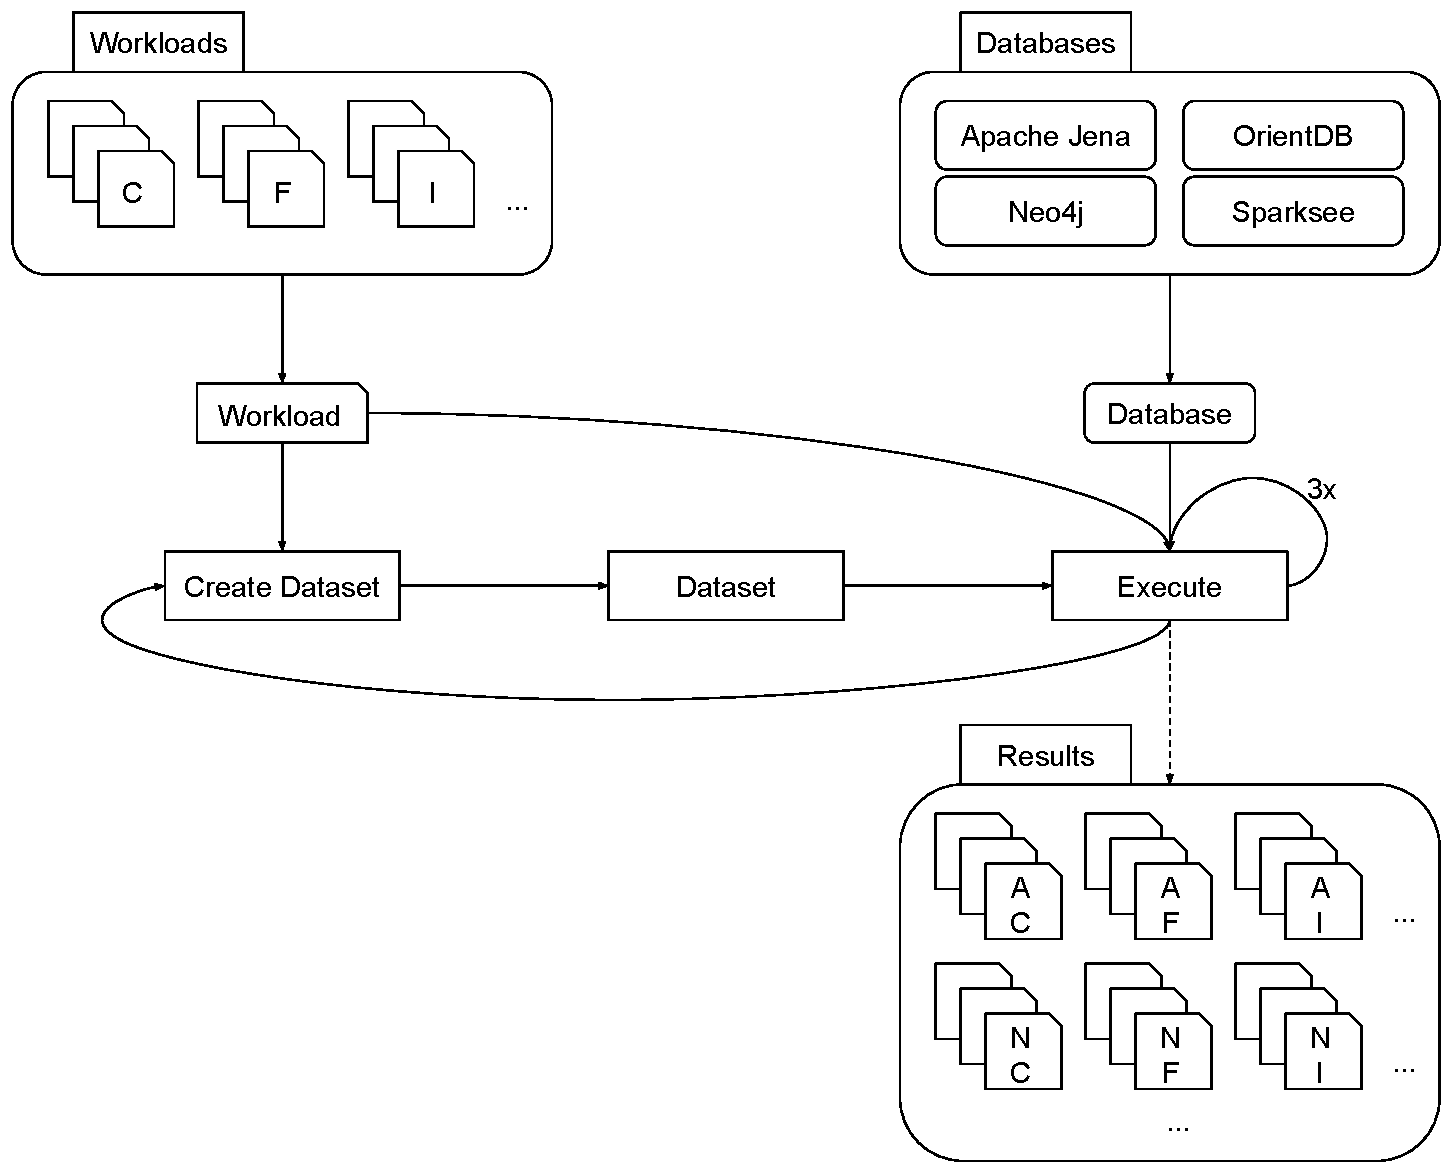
\includegraphics[width=\textwidth]{images/executionWorkflow}
  \caption{Workflow for the execution process.}
  \label{fig:executionWorkflow}
\end{figure}

In table~\ref{tab:throughputOverview} and~\ref{tab:productionOverview} the groups of workloads we are comparing with each other are shown.
The naming of the workloads is similar to the naming introduced in section~\ref{ch:design:se:workloads}.

\begin{landscape}
  \begin{table}
    \begin{minipage}{\hsize}
      \begin{tabularx}{\hsize}{ | l | l | l | l | X | }
        \hline
        Section & First workload & Other workload(s) & Units of measurement & Reason \\ \hline
        \ref{ch:evaluation:se:probingNodeCount} & 1. With Index & 2.-5. With Index & Inserts/second, total time, database size & The throughput in inserts/second will show if the databases slow down over time when they get filled up.
        The total time will show us,
        when the maximum dataset size is reached for each individual database in terms of reasonable execution time.\\ \hline
        \ref{ch:evaluation:se:probingNodeCount} & 1. Without Index & 2.-5. Without Index & Inserts/second & The throughput will show if the databases slow down as they get filled. \\ \hline
        \ref{ch:evaluation:se:probingNodeCount} & n.\footnote{the workload with the largest possible amount of nodes in terms of execution time.} With Index & n. Without Index & Inserts/second & To see how much time indexing takes up. \\ \hline
        \ref{ch:evaluation:se:probingNodeSize} & 1. Node Size & 2.-5. Node Size & Inserts/second, database size & We want to find the amount of data at which the databases are significantly slower.
        The database size of the different databases will show their storage efficiency. \\ \hline
        \ref{ch:evaluation:se:differenceEdges} & 1. No Edges & 2. No Edges & Inserts/second & Check if there is a benefit of an index if only nodes are inserted. \\ \hline
        \ref{ch:evaluation:se:differenceEdges} & n. With Index & 1. No Edges & Inserts/second & How much does inserting edges cost. \\ \hline
      \end{tabularx}
    \end{minipage}
    \caption{Overview for the throughput workloads \todo{remove reason and mention in evaluation}}
    \label{tab:throughputOverview}
  \end{table}
  \begin{table}
    \begin{minipage}{\hsize}
      \begin{tabularx}{\hsize}{ | l | l | l | l | X | }
        \hline
        Section & First workload & Other workload(s) & Units of measurement & Reason \\ \hline
        \ref{ch:evaluation:se:productComplexity} & 1. Structure & 2.-3. Structure & Inserts/second & Does the structure has an impact on performance. \\ \hline
        \ref{ch:evaluation:se:productionSuitability} & x.\footnote{Every workload will be evaluated} Suitablitiy & - & Total time & Check if the workload is completed faster then the production period it represents. \\ \hline
        \ref{ch:evaluation:se:retrievingUnderLoad} & 1. Reading & 2. Reading & Reads/second & Observe if there is a difference in using an index. \\ \hline
        \ref{ch:evaluation:se:retrievingUnderLoad} & 1. Scanning & 2. Scanning & Scans/second & See if there is a difference in using an index for scanning. \\ \hline
        \ref{ch:evaluation:se:retrievingUnderLoad} & 1. Structure & 1. Reading \& 1. Scanning & Operations/second & Investigate if other operations effect inserting data and compare operation throughput. \\ \hline
      \end{tabularx}
    \end{minipage}
    \caption{Overview for the production and retrieval workloads}
    \label{tab:productionOverview}
  \end{table}
\end{landscape}

After execution we have to combine the results for further inspection.
Figure~\ref{fig:evaluationWorkflow} illustrates this process of evaluation.
With all the results in one place we filtered the measurements for those we wanted,
then we calculated the average over the three benchmark runs we did with every database and workload.
Next we grouped the measurements as shown in tables~\ref{tab:throughputOverview} and~\ref{tab:productionOverview}.
Finally we created the diagrams shown in subsections "Results" of the following sections and interpreted them to draw a conclusion,
which is presented in the "Discussion" subsections.

\begin{figure}[!h]
  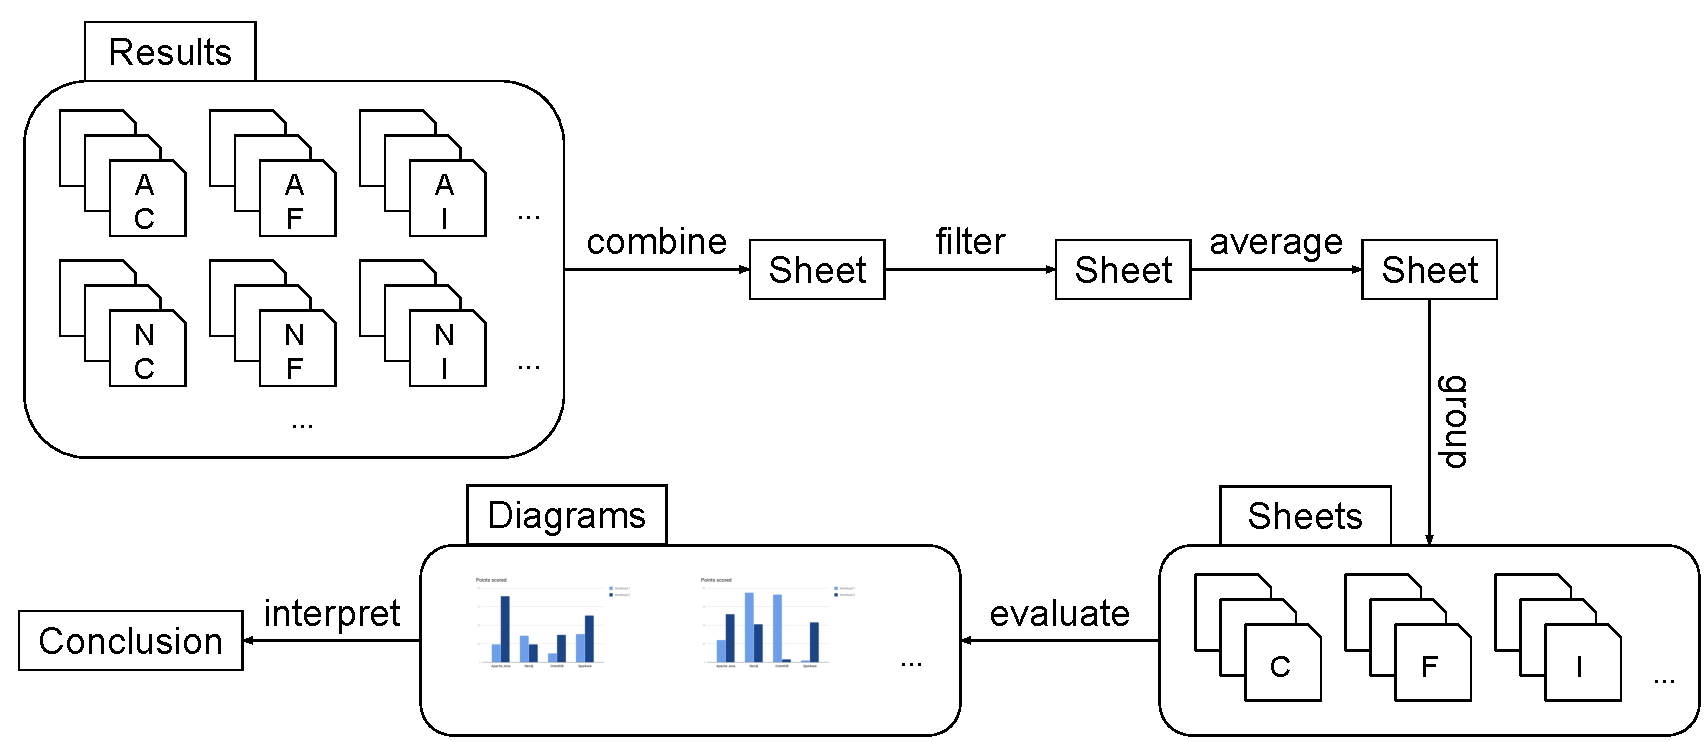
\includegraphics[width=\textwidth]{images/evaluationProcess}
  \caption{Workflow of the evaluation process.}
  \label{fig:evaluationWorkflow}
\end{figure}

\section{Throughput}
\label{ch:evaluation:se:throughput}
\todo{Tell at the beginning what we want to see. Insert includes edges, which have to look up nodes.}

In this section we will examine the combinations of workloads mentioned in table~\ref{tab:throughputOverview}.
The results from these workloads will give us an understanding of how the databases perform in terms of insertions per seconds depending on different factors.


\subsection{Probing Node Count}
\label{ch:evaluation:se:probingNodeCount}
Here we will compare how the throughput,
measured in inserts per second,
of the databases is effected by increasing the number of nodes we are inserting into it.
We will also look at the execution time,
to determine a reasonable large dataset in terms of execution time for the upcoming benchmark runs.

The throughput is listed in inserts per seconds,
which include both inserting nodes and inserting edges.
Note that in order to insert an edge the start and end node has to be looked up.

Apache Jena has no option to turn off indexing as mentioned in section~\ref{ch:background:se:apacheJena},
but it is still shown in the diagrams as reference.

\subsubsection{Results}
\todo{maybe include tables with numbers}
The first figure~\ref{fig:withIndexThroughput} shows how the different databases perform with an increasing dataset size.
Apache Jena and Neo4j only have values for 1.000 and 10.000 nodes,
because execution with more than 10.000 nodes would take too much time.
Sparksee only delivered results up to 100.000 nodes,
because the free license only included database sizes of up to 1.000.000 elements and a workload with 1.000.000 nodes would contain 2.333.333 elements in total with the edges.

In figure~\ref{fig:withIndexExecutionTime} we see the execution time of the different databases.
At 10.000 nodes Apache Jena and Neo4j took almost an hour for one run,
because of that we did not run it with 100.000 nodes or more.

\begin{figure}[h!]
  \centering
  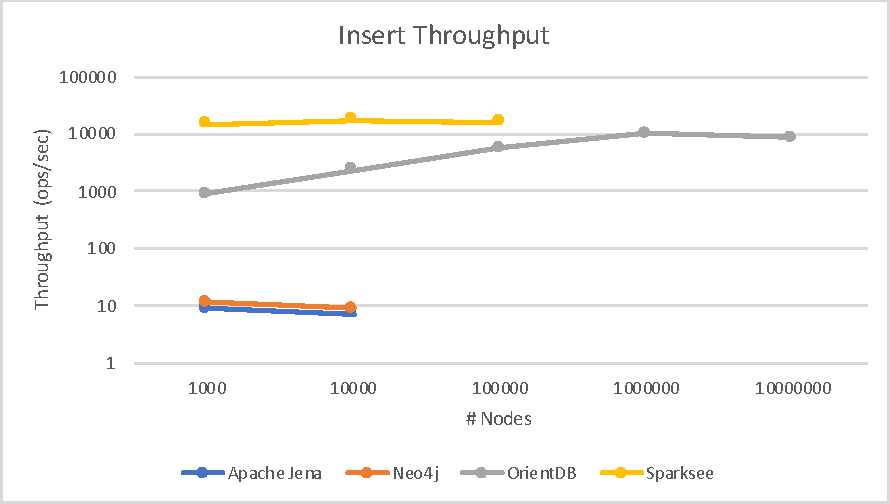
\includegraphics[width=.75\textwidth]{images/throughput/withIndexThroughput}
  \captionof{figure}{This figure shows the throughput in inserts/second of every database over different dataset sizes.}
  \label{fig:withIndexThroughput}
\end{figure}

\begin{figure}[h!]
  \centering
  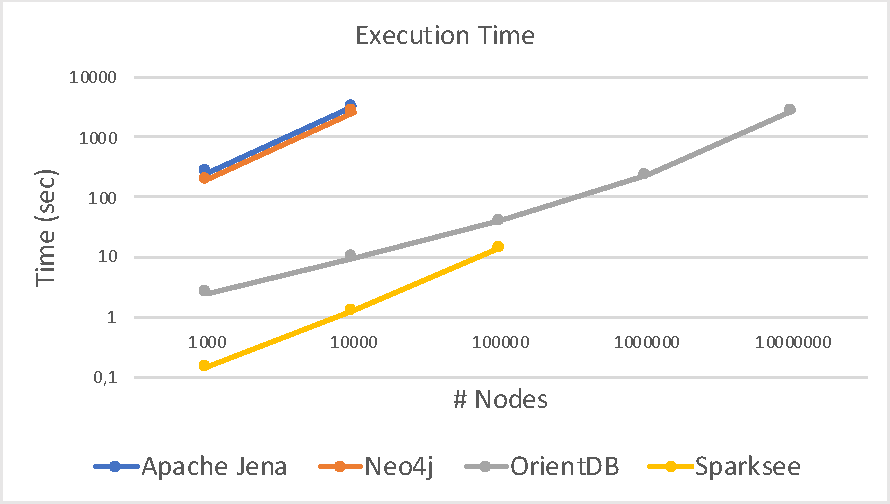
\includegraphics[width=.75\textwidth]{images/throughput/withIndexExecutionTime}
  \captionof{figure}{The execution time of the databases is shown over different dataset sizes.}
  \label{fig:withIndexExecutionTime}
\end{figure}

Figure~\ref{fig:withoutIndexThroughput} shows the throughput over different dataset sizes without using an index.
In figure~\ref{fig:withWithoutIndexThroughputFixNodes} we see a comparison of using an index and not with a dataset size of 10.000 nodes.

\begin{figure}[h!]
  \centering
  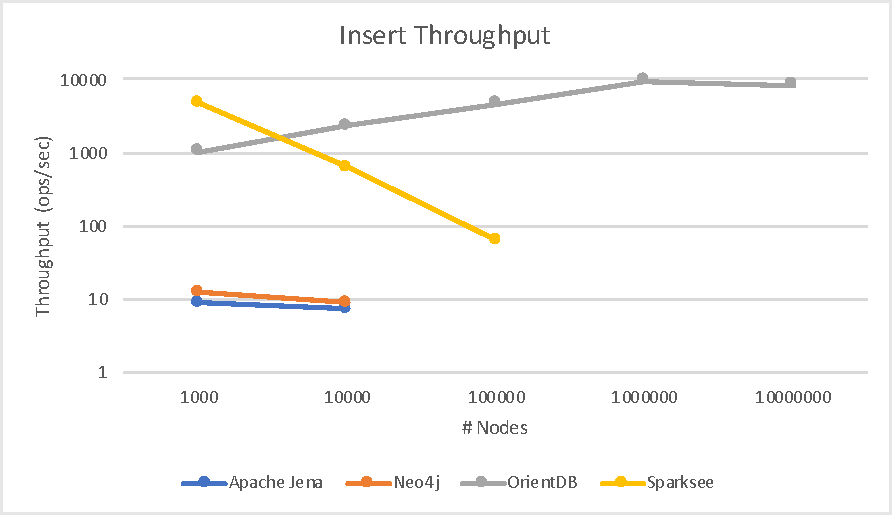
\includegraphics[width=.75\textwidth]{images/throughput/withoutIndexThroughput}
  \captionof{figure}{This diagram shows the throughput in inserts per second while using no index.}
  \label{fig:withoutIndexThroughput}
\end{figure}

\begin{figure}[h!]
  \centering
  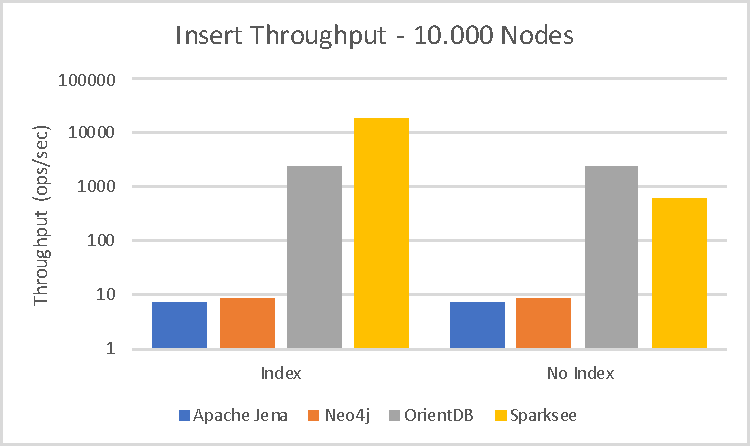
\includegraphics[width=.75\textwidth]{images/throughput/withWithoutIndexThroughputFixNodes}
  \captionof{figure}{The throughput at a fixed dataset size to compare between indexing and not.}
  \label{fig:withWithoutIndexThroughputFixNodes}
\end{figure}

\subsubsection{Discussion}
Figure~\ref{fig:withWithoutIndexThroughputFixNodes} shows us,
that there is no performance change for Jena, Neo4j and OrientDB in using an index or not.
Sparksee shows a significant drop in throughput without the use of an index.
That is what we expected,
because the throughput also contains insertions of edges,
which have to look up nodes,
what is faster with an index.
For the other databases the lack of difference in performance might by,
that the benefit of using an index to retrieve the nodes for an edge is equalised by the time they take to insert the nodes into the index.

The execution time grows linearly,
which is a good sign,
because that means that the databases do scale for larger amounts of data.

If we compare the archived throughput with out target throughput of \todo{calculate target throughput},
we see that Sparksee exceeds our target with $ 16435 \frac{inserts}{s} $.
OrientDB misses our goal slightly,
at the larges dataset it only archived a throughput of $ 8572 \frac{inserts}{s} $.
Jena and Neo4j didn't even reach $ 10 \frac{inserts}{s} $.
These throughput values are measured with another data structure and node size than the one we will use for the suitability workload,
so we will investigate the factors differentiating this workload from the suitability workload and reference these results again in section~\ref{ch:evaluation:se:suitabilityDiscussion}.

From these results alone,
without looking at read performance separately we can say,
that an index is useful,
even for insert operations,
because edges need to look up two nodes,
which is faster when an index is used.

\subsection{Probing Node Size}
\label{ch:evaluation:se:probingNodeSize}
In this subsection we will take a look at how the databases perform with different node property sizes.
We will pick a dataset size of 10.000 nodes,
as all database have a reasonable execution time with that amount of nodes.

By investigating the performance under node size variation,
we will see if the databases can store larger amount of data in one node.
That can be useful depending on the use case,
in our example given by the industry only a two digit number is stored,
but it could be desirable to store longer number or more complex information.

\subsubsection{Results}
In figure~\ref{fig:nodeSize} we see,
how an increasing node size has an impact on insert throughput.

Sparksee only has values for node sizes up to $ 1KB $,
because the property we used to store the value of the node only supports up to 2048 characters/Bytes.

Figure~\ref{fig:sizeDatabaseSize} shows the size of the database folder,
in which the database stores its files.

\begin{figure}[h!]
  \centering
  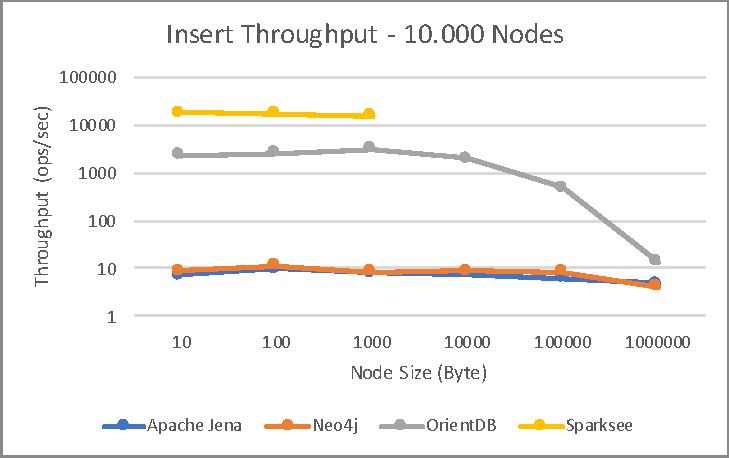
\includegraphics[width=.75\textwidth]{images/throughput/nodeSize}
  \captionof{figure}{Insert throughput over different node sizes with 10.000 nodes total.}
  \label{fig:nodeSize}
\end{figure}

\begin{figure}[h!]
  \centering
  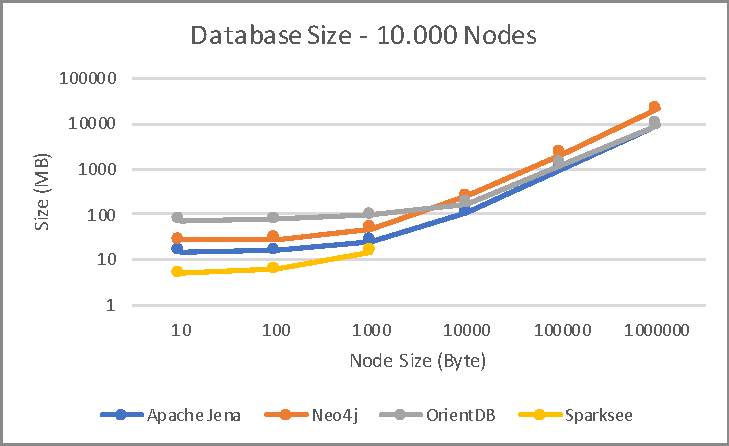
\includegraphics[width=.75\textwidth]{images/throughput/sizeDatabaseSize}
  \captionof{figure}{The size of the databases over growing node sizes.}
  \label{fig:sizeDatabaseSize}
\end{figure}

\subsubsection{Discussion}
Figure~\ref{fig:nodeSize} show that the throughput of Jena and Neo4j is quite low and it doesn't show much difference with larger node sizes,
but at $ 1MB $ we can see that the performance decreases even more.

For OrientDB we se good performance up to $ 1KB $,
it starts to decline for node sizes of $ 10KB $ and above with a significant drop at $ 1MB $.

Sparksee has the highest throughput of all four databases,
but as it could only handle sized of up to $ 2KB $ or $ 1KB $ in our test scenario.
In that range the other databases also show no noteworthy change in performance,
so we can't draw a conclusion about the behaviour of Sparksee with larger node sizes.

In figure~\ref{fig:sizeDatabaseSize} we see that the database size grows linearly with the node size,
from $ 10KB $ and above.
So for smaller node values the overhead of the database itself determines the size of the database.

When we look closely at the values of Neo4j,
we can see that they are above the other database.
In fact at $ 1MB $ node size,
which would result in $ 10GB $ data for 10.000 nodes,
Neo4js database folder had a size of $ 22GB $,
so the overhead is more than the data itself.

\subsection{Difference without Edges}
\label{ch:evaluation:se:differenceEdges}
Here we will investigate how the absents of edges has an impact on performance.
These workloads to not represent a real world scenario,
but they will provide us knowledge about how much inserting nodes costs compared to edges,
as for every edge its start and end node have to be looked up.

Apache Jena always uses an index,
but it is still shown in both parts of the diagram as reference.

\subsubsection{Results}
Figure~\ref{fig:noEdges} shows us the difference in using an index compared to not doing so,
while only inserting nodes.

\begin{figure}[h!]
  \centering
  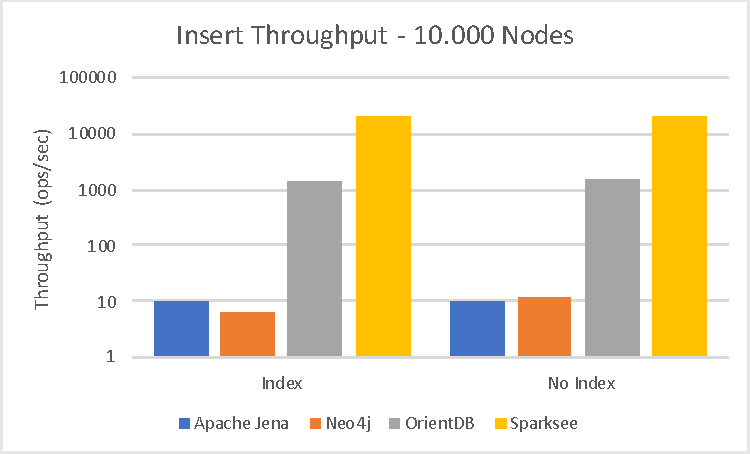
\includegraphics[width=.75\textwidth]{images/throughput/noEdges}
  \caption{Difference between using an index and not while using no edges.}
  \label{fig:noEdges}
\end{figure}

In figure~\ref{fig:indexNoEdges10000Nodes} we see a comparison of all databases between using edges and not with a dataset size of 10.000 nodes.
Figure~\ref{fig:indexNoEdges100000Nodes} shows a similar comparison with a bigger dataset,
but only between OrientDB and Sparksee,
as they were able to handle larger dataset within an acceptable time frame.

\begin{figure}[h!]
  \centering
  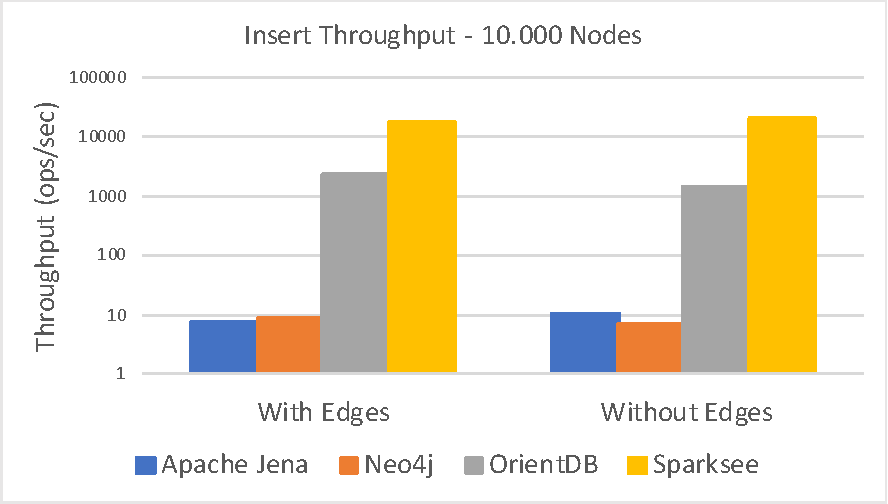
\includegraphics[width=.75\textwidth]{images/throughput/indexNoEdges10000Nodes}
  \captionof{figure}{Comparison of insert throughput between using edges and not.\newline}
  \label{fig:indexNoEdges10000Nodes}
\end{figure}

\begin{figure}[h!]
  \centering
  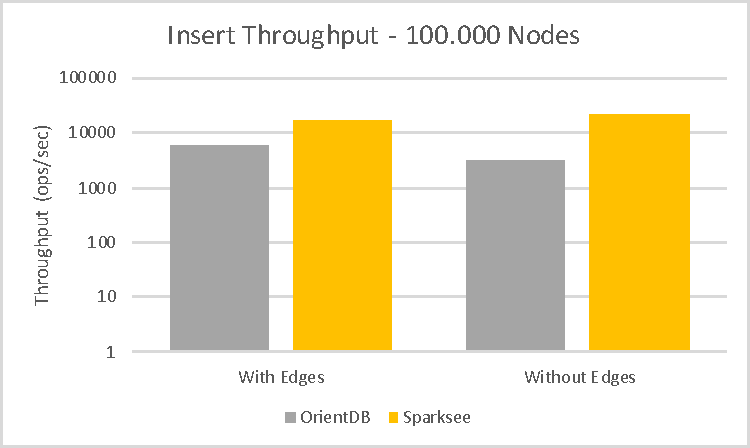
\includegraphics[width=.75\textwidth]{images/throughput/indexNoEdges100000Nodes}
  \captionof{figure}{Comparison of the insert throughput with 100.000 nodes between using edges and not.}
  \label{fig:indexNoEdges100000Nodes}
\end{figure}

\subsubsection{Discussion}
\todo{Do edges effect throughput}
As expected in figure~\ref{fig:noEdges} we can see,
that using an index does not benefit the insert performance for nodes.
Only Neo4j shows a notable difference for the node insert throughput with the use of an index the throughput drop to $ 6,6 \frac{inserts}{s} $ from $ 12 \frac{inserts}{s} $ without an index.

Figure~\ref{fig:indexNoEdges10000Nodes} shows,
that the insert throughput of Apache Jena is slightly lower when using edges.

\section{Production Simulation}
\label{ch:evaluation:se:productionSimulation}
The workload results presented in this section will cover the production specific variables.
The first one being product complexity and the other one execution time.

\subsection{Product Complexity}
\label{ch:evaluation:se:productComplexity}
\note{Structure has no effect, how the edges are connected between the nodes. But edges count matters as we see in comparison to the other benchmarks}
\todo{From Design: Number of edges could effect the throughput, because of inserts. social networks have much more edges to it than our structure}
If the throughput is not effected by using no edges compared to using edges,
we could see,
that for a graph database the structure of the data has no impact on performance.
This result is quite important,
as it would lead to the conclusion,
that we can use the results of other graph database benchmarks for our industrial use case.

The product complexity describes,
how much the tree representing our data structure is widened at three different levels shown in section~\ref{ch:design:se:dataStructure}.

The wider the data structure becomes the less edges we have per node.
That can be interesting if we want to compare the generalisation of the throughput with different graph structures,
which we need to determine if the throughput archived in section~\ref{ch:evaluation:se:probingNodeCount} can be used to draw conclusions about the suitability for the industrial environment.

\subsubsection{Results}
In figure~\ref{fig:structure} we see the impact a different data structure has on the insert throughput.

\begin{figure}[h!]
  \centering
  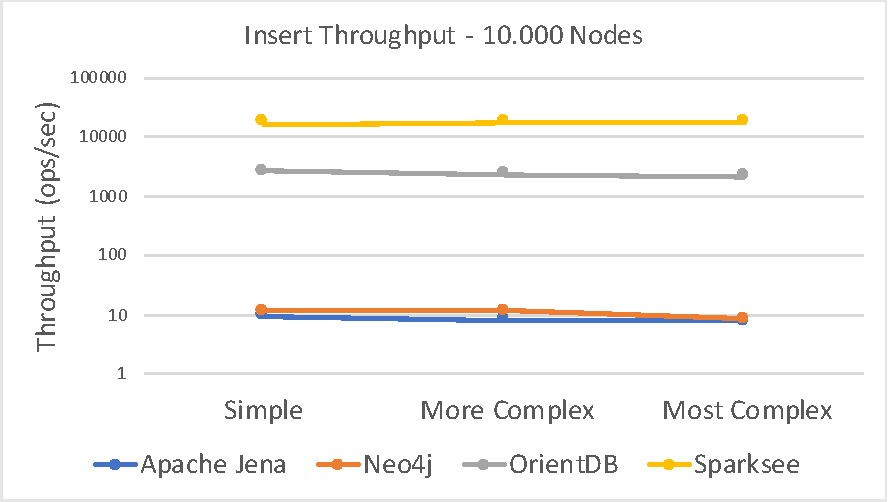
\includegraphics[width=.75\textwidth]{images/production/structure}
  \caption{Shows the difference in insert throughput over changing data structure.}
  \label{fig:structure}
\end{figure}

\subsubsection{Discussion}
As we see in figure~\ref{fig:structure} the structure of the data as we modelled it,
doesn't effect the throughput of the databases.

For the "simple" workload the have an edge to node ratio of around $ 1.33 $ which is dropping to $ ~1 $ for the "most complex" workload.
Together with the results from~\ref{ch:evaluation:se:differenceEdges} we can say,
that the use of edges has almost no impact on performance and the edge to node ratio also doesn't.

 draw a conclusion about the comparability with other related work using social network graphs,
which have a much higher edge to node ratio,
in order to do so we would have to investigate higher edge to node ratios.

\subsection{Production Suitability}
\label{ch:evaluation:se:productionSuitability}
The production simulations will finally show,
if the databases we chose are capable of storing the necessary amount of data in a specified time interval.

In the discussion of this section we will also investigate the throughput based on the previous workloads.

\subsubsection{Results}
Figure~\ref{fig:singleSuitability} show how long OrientDB took,
to store three minutes of production data (1.056.833 nodes).
Sparksee is mentioned with a theoretical time,
since it only allowed us to store 500.000 elements.
We took the throughput during inserting these 500.000 elements and calculated the time it would need to complete the whole workload.
The same was done for the results shown in figure~\ref{fig:hourSuitability}.

In figure~\ref{fig:hourSuitability} the same is shown but with a dataset that represents one hour of production,
which contains 21.136.660 nodes.

Only OrientDB and Sparksee were used in these workloads,
because Apache Jena and Neo4j would take too long to insert that amount of nodes.

\begin{figure}[h!]
  \centering
  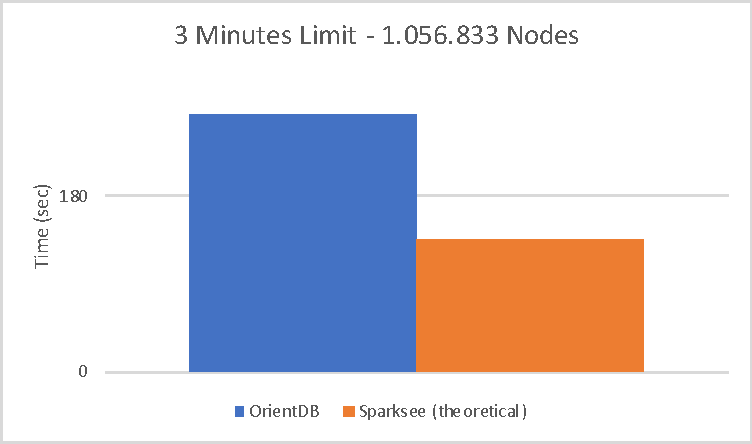
\includegraphics[width=.75\textwidth]{images/production/singleSuitability}
  \captionof{figure}{Shows the execution time with a dataset that represents three minutes of production.}
  \label{fig:singleSuitability}
\end{figure}

\begin{figure}[h!]
  \centering
  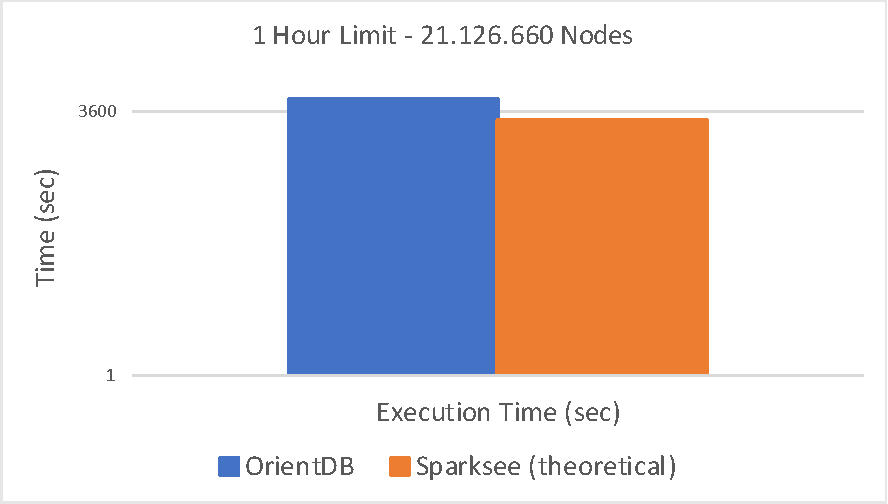
\includegraphics[width=.75\textwidth]{images/production/hourSuitability}
  \captionof{figure}{Shows the execution time with a dataset that represents one hour of production.}
  \label{fig:hourSuitability}
\end{figure}

\subsubsection{Discussion}
\label{ch:evaluation:se:suitabilityDiscussion}
The figures~\ref{fig:singleSuitability} and~\ref{fig:hourSuitability} show us,
that OrientDB did not manage to store the three minutes or the one hour of production simulation in the specified time.

Sparksee could theoretically store that amount without exceeding the time limit,
but since the free license did not allow for the amount of data we used the average util the limit was reached.
Of course it could be,
that the throughput of Sparksee drops with an increasing number of elements in the database,
but we couldn't investigate that.

The difference of this workload compared to the first workload we discussed in section~\ref{ch:evaluation:se:probingNodeCount} is the structure and the node size.
The results of~\ref{ch:evaluation:se:probingNodeSize} and~\ref{ch:evaluation:se:productComplexity} show,
that the structure has no impact on the throughput and the node size has no impact below $ 10KB $,
since we used $ 50B $ we can compare the first measured throughput.

By doing so we see that Sparksee,
again theoretically,
reaches our target throughput of $ 11743 \frac{inserts}{s} $.
OrientDB misses our target with $ 8572 \frac{inserts}{s} $.
These results support our findings for the impact of structure and node size,
as this workload,
measuring the time correlates with the numbers from the first workload.

\section{Retrieving under load}
\label{ch:evaluation:se:retrievingUnderLoad}
\todo{compare to results of other studies}
This section will cover the results about retrieving data while the database is under load.
First we will take a look at how using an index is effecting the read and scan throughput,
then we will compare the throughput of the different operations~(\ref{fig:operationReadScan}) and their impact on the insert operation~(\ref{fig:insertWithWithoutReadScan}).

\subsection{Results}
In figure~\ref{fig:readThroughput10000Nodes} and~\ref{fig:scanThroughput10000Nodes} we see the throughput of read and scan operations when using an index or not.

\begin{figure}[h!]
  \centering
  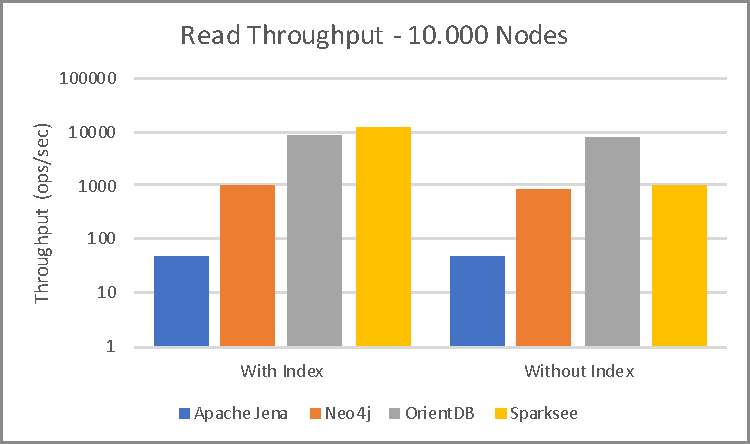
\includegraphics[width=.75\textwidth]{images/responsiveness/readThroughput10000Nodes}
  \captionof{figure}{Shows the throughput of read operations with and without the use of an index.}
  \label{fig:readThroughput10000Nodes}
\end{figure}

\begin{figure}[h!]
  \centering
  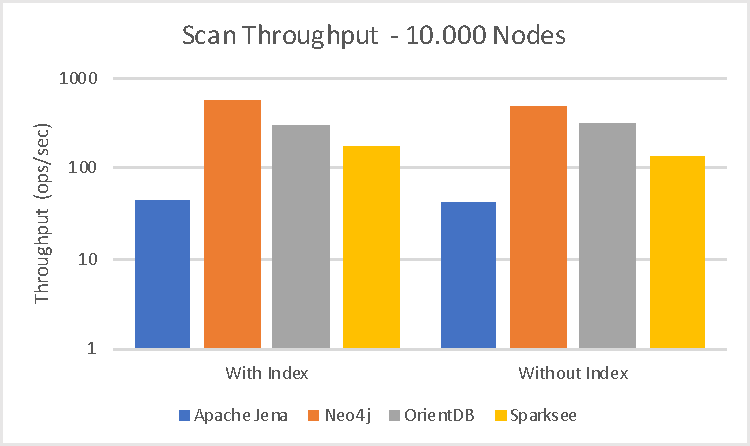
\includegraphics[width=.75\textwidth]{images/responsiveness/scanThroughput10000Nodes}
  \captionof{figure}{Shows the throughput of read operations with and without the use of an index.}
  \label{fig:scanThroughput10000Nodes}
\end{figure}

Figure~\ref{fig:operationReadScan} shows the throughput of the different operations.
In figure~\ref{fig:insertWithWithoutReadScan} we see the impact of the read and scan operations on the insert operations.

\begin{figure}[h!]
  \centering
  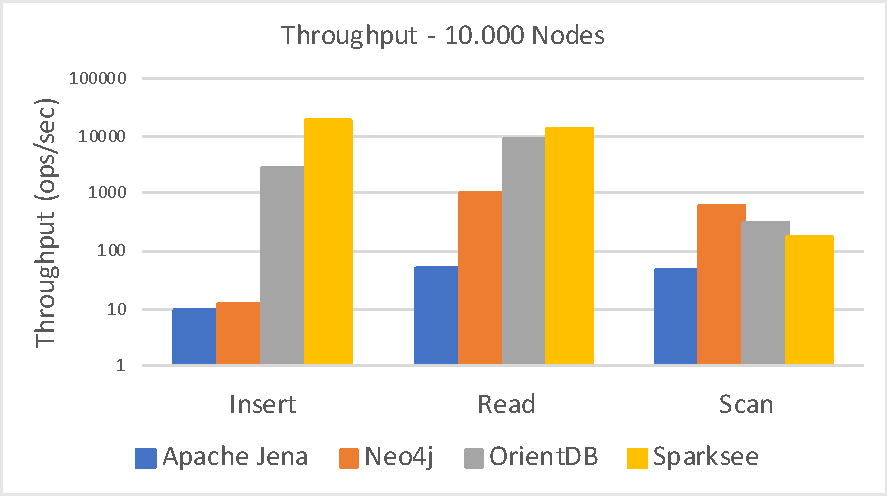
\includegraphics[width=.75\textwidth]{images/responsiveness/operationReadScan}
  \captionof{figure}{Shows the throughput of the different operations.\newline}
  \label{fig:operationReadScan}
\end{figure}

\begin{figure}[h!]
  \centering
  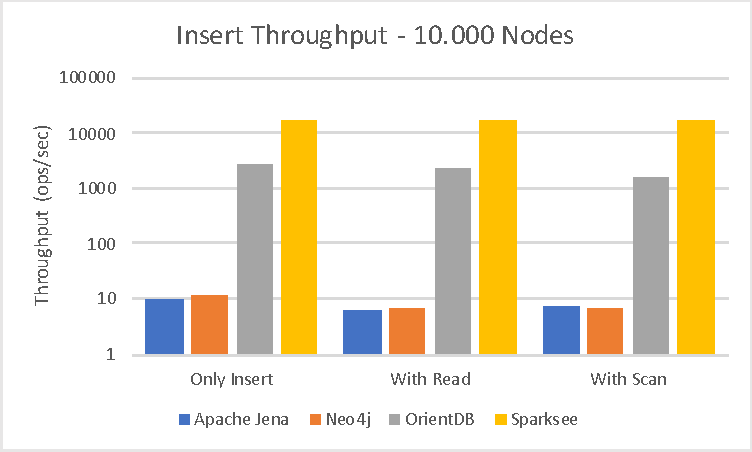
\includegraphics[width=.75\textwidth]{images/responsiveness/insertWithWithoutReadScan}
  \captionof{figure}{Shows the throughput of insert operations when using different operations.}
  \label{fig:insertWithWithoutReadScan}
\end{figure}

\subsection{Discussion}
First we will discuss the results regarding the use of an index and not.
For read operations figure~\ref{fig:readThroughput10000Nodes} shows,
that all databases benefit from using an index,
except Apache Jena which always uses an index and is only presented as reference.
Sparksee shows the biggest difference in throughput of read operations,
whereas the others only show a slight decrease in performance without an index.
That was what we would expect,
since an index really benefits these kinds of operations,
although we expected the increase with the use of an index to be higher for Neo4j and OrientDB.
It could be,
that the dataset size is too small to show an effect between using an index and not.

Similar results can be seen for the scan operations shown in figure~\ref{fig:scanThroughput10000Nodes}.
The absence of an index has not much effect here either,
that could be the case,
because scan operations only use one read operations for the start node and then traverse the graph,
which is not effected by the index.

The comparison of the different operations shown in figure~\ref{fig:operationReadScan} shows us where the strengths and weaknesses are in the different databases.
Apache Jena and Neo4j are the slowest when it comes to inserting nodes,
but they are much faster in retrieving nodes,
with Neo4j even being the fastest of all four in graph traversal.

OrientDB and Sparksee seem to be a good choice then inserting and reading is the main concern of the application.

When we compare the results of Apache Jena from its read performance to its scan performance,
we see almost no difference in performance,
which means it is even faster than Neo4j in graph traversal,
but it is limited by the relatively slow read operation at the beginning of the scan operation.

The last figure~\ref{fig:insertWithWithoutReadScan} shows us,
that using other operations on the database does effect insert throughput,
except for Sparksee,
which seems to stay stable in its throughput even when other operations are being used.

Jena and Neo4j are low in throughput anyways,
but they still suffer from other operations being executed regularly.
OrientDB has a slightly worse throughput when using read operations and even worse with scan operations,
that is not good for our industry scenario,
because in the industry read and scan operations will be used in the database more or less regularly,
depending on the specific use case.

\section{Related Work and Generalisability}
\label{ch:evaluation:se:relatedWorkAndGeneralisability}
In this section we will compare our results with the findings of our related work as it's suitable.
Our main goal is to investigate if the difference in structure has an impact on performance,
when that is not the case we can assume,
that benchmark results from research on social network graph can be used to evaluate the performance of a graph database in an industrial environment.
The key point we will investigate is how the number of edges in relation to the number of nodes effects the throughput performance of the databases,
as for social network graphs that number is quite high at around $ 8 $\cite[41]{TaoShen} to $ 22 $\cite{Dayarathna2012} whereas our graph structure contains a edge to node ratio of $ 1.3 $ to $ ~1 $ (depending on the variables x, y and z; higher variable values lead to a ratio closer to 1).

By comparing our finding with the ones from Dominguez-Sal et al.\cite{TaoShen} which can be seen in figure~\ref{fig:throughputShen} we see,
that all databases performed much better than in our experiment.
The throughput of Neo4j and Jena is well above $ 100 \frac{inserts}{s} $ and Sparksee too reaches a higher throughput with $ 29770 \frac{inserts}{s} $.
This higher performance could be the results from a lack of information stored in the nodes,
as the paper only mentions weights on the inserted edges we cannot surely tell if that is the case.
With that in mind we can come to the conclusion,
that databases perform worse in an industrial environment and the results of graph database benchmarks cannot be transferred into the industrial context,
as we can't tell how much throughput is sacrificed by storing information in the nodes.

\begin{figure}[!h]
  \centering
  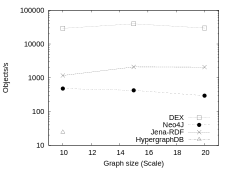
\includegraphics[width=.8\textwidth]{images/benchmarks/ShenResultsInsert}
  \caption{Throughput results from Dominguez-Sal et al.\cite{TaoShen}}
  \label{fig:throughputShen}
\end{figure}

The research of Dayarathna et al.\cite{Dayarathna2012} used a edge to node ration of 22 with a node count of 1024.
Comparing their results shown in figure~\ref{fig:throughputXGDBench} with our results from figure~\ref{fig:withIndexThroughput} lead to the conclusion,
that the databases perform better with an industrial graph structure and less edges.
The throughput of OrientDB is split in half compared to our workload at the almost same amount of nodes (1024 vs. 1000 in our research).
With this observation we come to the conclusion that graph databases would perform even better in an industrial environment,
but since the dataset size which we can compare is too small we cannot surely tell if that holds true for larger node counts.

\begin{figure}[!h]
  \centering
  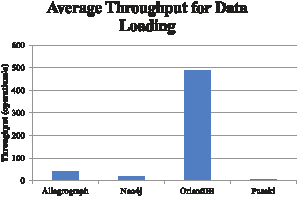
\includegraphics[width=\textwidth]{images/benchmarks/XGDBenchResultsInsert}
  \caption{Throughput results from the XGDBench Benchmark\cite{Dayarathna2012}}
  \label{fig:throughputXGDBench}
\end{figure}

If we look at our own findings in figure~\ref{fig:indexNoEdges10000Nodes} we can come to the conclusion that the throughput is better when using edges,
which correlates with the comparison to the research conducted by Dominguez-Sal,
but the throughput becomes even better as the number of edges compared to the number of nodes increases and as the ratio of edges to nodes is relatively low in an industrial application that again leads the conclusion,
that graph databases perform worse in the industrial environment and the results of graph benchmarks cannot not be used to determine performance in the industrial internet of things.
        % Evaluierung
\chapter{Conclusion and Future Work}
\label{ch:futureWork}
After conducting our experiments and evaluating the results we will finally end with a conclusion and give ideas for future research in this field.
At the end we will summarise the research we have done.

\section{Conclusion}
\label{ch:futureWork:se:conclusion}
In this section we will draw a conclusion regarding the suitability for the industrial data space and the generalisability of graph benchmarking results measured with social graphs.

\subsection{Suitability}
From our findings we can say,
that no database is able to store the necessary amount of data as we dimensioned within the corresponding time frame.

Sparksee could be capable of handling our calculated amount,
but we couldn't test it at scale,
because of its license limitations.

\subsection{Generalisability}
With our results and the comparison with other research in this field,
we can say that the throughput of a graph database depends not only on the insert performance,
but among others,
also on read throughput as this is needed to insert edges into the database.\\
It is indirectly possible to transfer the throughput measured on social network graphs to throughput in an industrial application,
by taking the read throughput relative to the insert throughput into account and minding the data structure in particular the edge to node ratio.\\
Besides that, there are other factors effecting throughput as our comparison in section~\ref{ch:evaluation:se:relatedWorkAndGeneralisability} shows.

\section{Future Work}
As our investigations on the throughput of graph databases with data from the industrial internet of things couldn't lead to a solid conclusion about the comparability between performance results measured with social network graphs and industrial graphs,
a study should be conducted that investigates the impact of different edge to node ratios covering also different graph properties as the clustering coefficient for example to evaluate which graph properties effect the throughput of graph databases in which way.

\section{Summary}
The purpose of this research was to investigate the suitability of current graph databases for the use in an industrial environment and furthermore examine if the results from previous research conducted in the field of graph database benchmarking can be generalised to be applied on the industrial use case.\\
To do so available database benchmarks have been looked up alongside with graph databases analysed in other studies.
A lack of results for the industrial data space was found and a data structure was created to represent the industrial use case for a graph database and an available benchmark was extended to produce datasets with that structure.
Workloads were designed to mirror the use of a graph database in an industrial environment.
After executing the workloads with the designed data structure of the graph databases,
their throughput under different situations was measured and compared with other studies.

The results show that most current databases aren't suitable for use in the industry.
Sparksee was the only database able to reach the target throughput for insert operations.
OrientDB missed our target only slightly,
whereas Apache Jena and Neo4j are far from being able to store that amount of data in the specified time.

From the results no clear conclusion can be made about the generalisation of benchmark results of graph databases,
as the result of comparison with other research points in opposite directions.
However more arguments suggest,
that graph databases perform worse in an industrial application and therefore the results of other studies cannot be applied to determine the performance of a graph database in an industrial environment.
  % Future Work
%\chapter{Summary}
\label{ch:Summary}
   % Zusammenfassung und Ausblick

%% ++++++++++++++++++++++++++++++++++++++++++
%% Anhang
%% ++++++++++++++++++++++++++++++++++++++++++

\appendix
%\include{anhang_a}
%\include{anhang_b}

%% ++++++++++++++++++++++++++++++++++++++++++
%% Literatur
%% ++++++++++++++++++++++++++++++++++++++++++
%  mit dem Befehl \nocite werden auch nicht
%  zitierte Referenzen abgedruckt
\cleardoublepage
\phantomsection
\addcontentsline{toc}{chapter}{\bibname}
%%
%\nocite{*} % nur angeben, wenn auch nicht im Text zitierte Quellen
           % erscheinen sollen
%\bibliographystyle{itmabbrv} % mit abgekürzten Vornamen der Autoren
%\bibliographystyle{gerplain} % abbrvnat unsrtnat
% spezielle Zitierstile: Labels mit vier Buchstaben und Jahreszahl
%\bibliographystyle{itmalpha}  % ausgeschriebene Vornamen der Autoren
\printbibliography
%% ++++++++++++++++++++++++++++++++++++++++++
%% Index
%% ++++++++++++++++++++++++++++++++++++++++++
\ifnotdraft{
\cleardoublepage
\phantomsection
\printindex            % Index, Stichwortverzeichnis
}
\end{document}
%% end of file
